\INEchaptercarta{Alumnos en preprimaria}{}



\cajita{Inscritos }{El número de  inscritos en preprimaria se obtiene a partir del total de los alumnos sin importar la edad, registrados al treinta de marzo de cada ciclo escolar\llamada. \textollamada{También se le llama estadística inicial} 
	
	En el 2009 se inscribieron 584,833 alumnos y en el 2013 se inscribieron 543,226 alumnos, lo cual representa un incremento del 13.7\%.}{Número de inscritos en el ciclo de educación preprimaria}{República de Guatemala, serie histórica, en datos absolutos}{\ \\[0mm]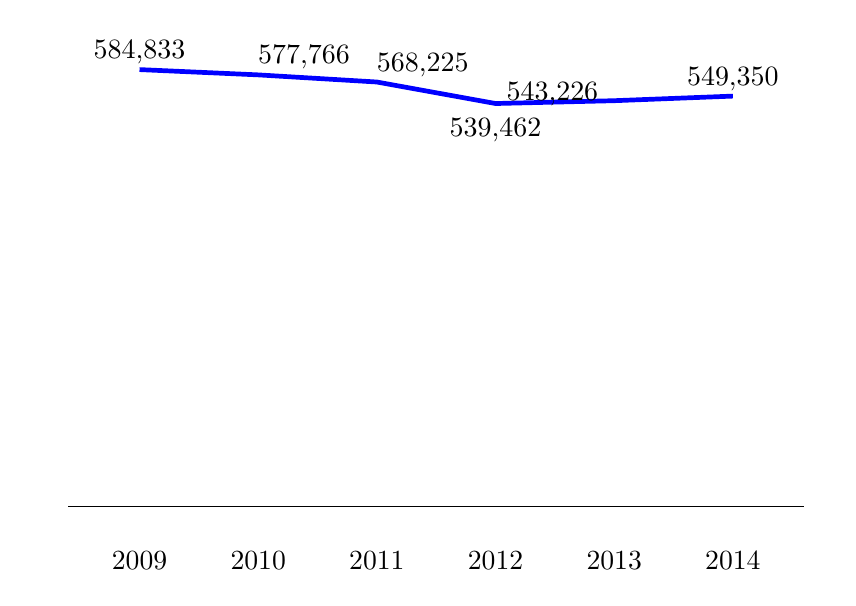
\begin{tikzpicture}[x=1pt,y=1pt]  % Created by tikzDevice version 0.8.1 on 2015-12-10 16:25:19
% !TEX encoding = UTF-8 Unicode
\definecolor{fillColor}{RGB}{255,255,255}
\path[use as bounding box,fill=fillColor,fill opacity=0.00] (0,0) rectangle (289.08,198.74);
\begin{scope}
\path[clip] (  0.00,  0.00) rectangle (289.08,198.74);

\path[] (  0.00,  0.00) rectangle (289.08,198.74);
\end{scope}
\begin{scope}
\path[clip] (  0.00,  0.00) rectangle (289.08,198.74);

\path[] ( 14.70, 17.78) rectangle (280.54,191.48);

\path[] ( 14.70, 52.66) --
	(280.54, 52.66);

\path[] ( 14.70,106.67) --
	(280.54,106.67);

\path[] ( 14.70,160.68) --
	(280.54,160.68);

\path[] ( 14.70, 25.65) --
	(280.54, 25.65);

\path[] ( 14.70, 79.66) --
	(280.54, 79.66);

\path[] ( 14.70,133.67) --
	(280.54,133.67);

\path[] ( 14.70,187.68) --
	(280.54,187.68);

\path[] ( 40.42, 17.78) --
	( 40.42,191.48);

\path[] ( 83.30, 17.78) --
	( 83.30,191.48);

\path[] (126.18, 17.78) --
	(126.18,191.48);

\path[] (169.06, 17.78) --
	(169.06,191.48);

\path[] (211.94, 17.78) --
	(211.94,191.48);

\path[] (254.82, 17.78) --
	(254.82,191.48);
\definecolor{drawColor}{RGB}{0,0,255}

\path[draw=drawColor,line width= 1.7pt,line join=round] ( 40.42,183.59) --
	( 83.30,181.68) --
	(126.18,179.10) --
	(169.06,171.33) --
	(211.94,172.35) --
	(254.82,174.01);
\definecolor{drawColor}{RGB}{0,0,0}

\node[text=drawColor,anchor=base,inner sep=0pt, outer sep=0pt, scale=  1.01] at ( 40.42,187.54) {584,833};

\node[text=drawColor,anchor=base west,inner sep=0pt, outer sep=0pt, scale=  1.01] at ( 83.30,185.64) {577,766};

\node[text=drawColor,anchor=base west,inner sep=0pt, outer sep=0pt, scale=  1.01] at (126.18,183.06) {568,225};

\node[text=drawColor,anchor=base,inner sep=0pt, outer sep=0pt, scale=  1.01] at (169.06,159.46) {539,462};

\node[text=drawColor,anchor=base east,inner sep=0pt, outer sep=0pt, scale=  1.01] at (206.16,172.35) {543,226};

\node[text=drawColor,anchor=base,inner sep=0pt, outer sep=0pt, scale=  1.01] at (254.82,177.96) {549,350};

\path[draw=drawColor,line width= 0.1pt,line join=round] ( 14.70, 25.67) -- (280.54, 25.67);

\path[] ( 14.70, 17.78) rectangle (280.54,191.48);
\end{scope}
\begin{scope}
\path[clip] (  0.00,  0.00) rectangle (289.08,198.74);

\path[] ( 14.70, 17.78) --
	( 14.70,191.48);
\end{scope}
\begin{scope}
\path[clip] (  0.00,  0.00) rectangle (289.08,198.74);
\definecolor{drawColor}{RGB}{255,255,255}

\node[text=drawColor,text opacity=0.00,anchor=base east,inner sep=0pt, outer sep=0pt, scale=  1.00] at (  7.58, 21.75) {0e+00};

\node[text=drawColor,text opacity=0.00,anchor=base east,inner sep=0pt, outer sep=0pt, scale=  1.00] at (  7.58, 75.76) {2e+05};

\node[text=drawColor,text opacity=0.00,anchor=base east,inner sep=0pt, outer sep=0pt, scale=  1.00] at (  7.58,129.77) {4e+05};

\node[text=drawColor,text opacity=0.00,anchor=base east,inner sep=0pt, outer sep=0pt, scale=  1.00] at (  7.58,183.77) {6e+05};
\end{scope}
\begin{scope}
\path[clip] (  0.00,  0.00) rectangle (289.08,198.74);

\path[] ( 10.43, 25.65) --
	( 14.70, 25.65);

\path[] ( 10.43, 79.66) --
	( 14.70, 79.66);

\path[] ( 10.43,133.67) --
	( 14.70,133.67);

\path[] ( 10.43,187.68) --
	( 14.70,187.68);
\end{scope}
\begin{scope}
\path[clip] (  0.00,  0.00) rectangle (289.08,198.74);

\path[] ( 14.70, 17.78) --
	(280.54, 17.78);
\end{scope}
\begin{scope}
\path[clip] (  0.00,  0.00) rectangle (289.08,198.74);

\path[] ( 40.42, 13.51) --
	( 40.42, 17.78);

\path[] ( 83.30, 13.51) --
	( 83.30, 17.78);

\path[] (126.18, 13.51) --
	(126.18, 17.78);

\path[] (169.06, 13.51) --
	(169.06, 17.78);

\path[] (211.94, 13.51) --
	(211.94, 17.78);

\path[] (254.82, 13.51) --
	(254.82, 17.78);
\end{scope}
\begin{scope}
\path[clip] (  0.00,  0.00) rectangle (289.08,198.74);
\definecolor{drawColor}{RGB}{0,0,0}

\node[text=drawColor,anchor=base,inner sep=0pt, outer sep=0pt, scale=  1.00] at ( 40.42,  2.85) {2009};

\node[text=drawColor,anchor=base,inner sep=0pt, outer sep=0pt, scale=  1.00] at ( 83.30,  2.85) {2010};

\node[text=drawColor,anchor=base,inner sep=0pt, outer sep=0pt, scale=  1.00] at (126.18,  2.85) {2011};

\node[text=drawColor,anchor=base,inner sep=0pt, outer sep=0pt, scale=  1.00] at (169.06,  2.85) {2012};

\node[text=drawColor,anchor=base,inner sep=0pt, outer sep=0pt, scale=  1.00] at (211.94,  2.85) {2013};

\node[text=drawColor,anchor=base,inner sep=0pt, outer sep=0pt, scale=  1.00] at (254.82,  2.85) {2014};
\end{scope}
  \end{tikzpicture}}{Instituto Nacional de Estadística, con datos del Ministerio de Educación}

\cajita{Inscritos por sexo}{La distribución de alumnos inscritos en educación preprimaria según su sexo, muestra que el 50.5\% fueron hombres, mayor en 1 punto porcentual respecto a las mujeres.}{Distribución de inscritos en el ciclo de\\ educación preprimaria, por sexo}{República de Guatemala, año 2013, en porcentaje}{\ \\[0mm]\begin{tikzpicture}[x=1pt,y=1pt]  % Created by tikzDevice version 0.10.1 on 2016-02-29 12:41:01
% !TEX encoding = UTF-8 Unicode
\definecolor{fillColor}{RGB}{255,255,255}
\path[use as bounding box,fill=fillColor,fill opacity=0.00] (0,0) rectangle (289.08,198.74);
\begin{scope}
\path[clip] ( 30.54,  0.00) rectangle (258.54,198.74);

\path[] ( 30.54,  0.00) rectangle (258.54,198.74);
\end{scope}
\begin{scope}
\path[clip] (  0.00,  0.00) rectangle (289.08,198.74);

\path[] (  7.11,  4.95) rectangle (200.91,198.74);

\path[] (104.01,101.85) --
	(191.21,100.67);

\path[] (104.01,101.85) --
	( 16.81,103.03);

\path[] (104.01,101.85) --
	(105.19,189.04);

\path[] (104.01,101.85) --
	(191.21,100.67);

\path[] (104.01,101.85) --
	(102.83, 14.65);

\path[] (104.01,101.85) --
	( 16.81,103.03);

\path[] (104.01,101.85) --
	(104.01,101.85) --
	(104.01,101.85) --
	(104.01,101.85) --
	(104.01,101.85) --
	(104.01,101.85) --
	(104.01,101.85) --
	(104.01,101.85) --
	(104.01,101.85) --
	(104.01,101.85) --
	(104.01,101.85) --
	(104.01,101.85) --
	(104.01,101.85) --
	(104.01,101.85) --
	(104.01,101.85) --
	(104.01,101.85) --
	(104.01,101.85) --
	(104.01,101.85) --
	(104.01,101.85) --
	(104.01,101.85) --
	(104.01,101.85) --
	(104.01,101.85) --
	(104.01,101.85) --
	(104.01,101.85) --
	(104.01,101.85) --
	(104.01,101.85) --
	(104.01,101.85) --
	(104.01,101.85) --
	(104.01,101.85) --
	(104.01,101.85) --
	(104.01,101.85) --
	(104.01,101.85) --
	(104.01,101.85) --
	(104.01,101.85) --
	(104.01,101.85) --
	(104.01,101.85) --
	(104.01,101.85) --
	(104.01,101.85) --
	(104.01,101.85) --
	(104.01,101.85) --
	(104.01,101.85) --
	(104.01,101.85) --
	(104.01,101.85) --
	(104.01,101.85) --
	(104.01,101.85) --
	(104.01,101.85) --
	(104.01,101.85) --
	(104.01,101.85) --
	(104.01,101.85) --
	(104.01,101.85) --
	(104.01,101.85) --
	(104.01,101.85) --
	(104.01,101.85) --
	(104.01,101.85) --
	(104.01,101.85) --
	(104.01,101.85) --
	(104.01,101.85) --
	(104.01,101.85) --
	(104.01,101.85) --
	(104.01,101.85) --
	(104.01,101.85) --
	(104.01,101.85) --
	(104.01,101.85) --
	(104.01,101.85) --
	(104.01,101.85) --
	(104.01,101.85) --
	(104.01,101.85) --
	(104.01,101.85) --
	(104.01,101.85) --
	(104.01,101.85) --
	(104.01,101.85) --
	(104.01,101.85) --
	(104.01,101.85) --
	(104.01,101.85) --
	(104.01,101.85) --
	(104.01,101.85) --
	(104.01,101.85) --
	(104.01,101.85) --
	(104.01,101.85) --
	(104.01,101.85) --
	(104.01,101.85) --
	(104.01,101.85) --
	(104.01,101.85) --
	(104.01,101.85) --
	(104.01,101.85) --
	(104.01,101.85) --
	(104.01,101.85) --
	(104.01,101.85) --
	(104.01,101.85) --
	(104.01,101.85) --
	(104.01,101.85) --
	(104.01,101.85) --
	(104.01,101.85) --
	(104.01,101.85) --
	(104.01,101.85) --
	(104.01,101.85) --
	(104.01,101.85) --
	(104.01,101.85) --
	(104.01,101.85) --
	(104.01,101.85);

\path[] (104.01,121.23) --
	(105.24,121.19) --
	(106.46,121.07) --
	(107.68,120.88) --
	(108.88,120.60) --
	(110.06,120.26) --
	(111.21,119.84) --
	(112.34,119.34) --
	(113.43,118.78) --
	(114.49,118.15) --
	(115.50,117.45) --
	(116.47,116.69) --
	(117.38,115.87) --
	(118.25,115.00) --
	(119.05,114.07) --
	(119.80,113.09) --
	(120.48,112.06) --
	(121.09,111.00) --
	(121.64,109.90) --
	(122.11,108.76) --
	(122.51,107.60) --
	(122.84,106.42) --
	(123.09,105.21) --
	(123.27,103.99) --
	(123.37,102.77) --
	(123.39,101.54) --
	(123.33,100.31) --
	(123.19, 99.09) --
	(122.98, 97.88) --
	(122.69, 96.68) --
	(122.32, 95.51) --
	(121.88, 94.36) --
	(121.37, 93.24) --
	(120.79, 92.16) --
	(120.14, 91.11) --
	(119.43, 90.11) --
	(118.66, 89.16) --
	(117.82, 88.25) --
	(116.93, 87.40) --
	(115.99, 86.61) --
	(115.00, 85.88) --
	(113.96, 85.22) --
	(112.89, 84.62) --
	(111.78, 84.09) --
	(110.64, 83.64) --
	(109.47, 83.25) --
	(108.28, 82.94) --
	(107.07, 82.71) --
	(105.85, 82.55) --
	(104.62, 82.48) --
	(103.39, 82.48) --
	(102.17, 82.55) --
	(100.95, 82.71) --
	( 99.74, 82.94) --
	( 98.55, 83.25) --
	( 97.38, 83.64) --
	( 96.24, 84.09) --
	( 95.13, 84.62) --
	( 94.05, 85.22) --
	( 93.02, 85.88) --
	( 92.03, 86.61) --
	( 91.09, 87.40) --
	( 90.20, 88.25) --
	( 89.36, 89.16) --
	( 88.59, 90.11) --
	( 87.87, 91.11) --
	( 87.23, 92.16) --
	( 86.65, 93.24) --
	( 86.13, 94.36) --
	( 85.70, 95.51) --
	( 85.33, 96.68) --
	( 85.04, 97.88) --
	( 84.83, 99.09) --
	( 84.69,100.31) --
	( 84.63,101.54) --
	( 84.65,102.77) --
	( 84.75,103.99) --
	( 84.92,105.21) --
	( 85.18,106.42) --
	( 85.50,107.60) --
	( 85.91,108.76) --
	( 86.38,109.90) --
	( 86.93,111.00) --
	( 87.54,112.06) --
	( 88.22,113.09) --
	( 88.97,114.07) --
	( 89.77,115.00) --
	( 90.64,115.87) --
	( 91.55,116.69) --
	( 92.52,117.45) --
	( 93.53,118.15) --
	( 94.59,118.78) --
	( 95.68,119.34) --
	( 96.81,119.84) --
	( 97.96,120.26) --
	( 99.14,120.60) --
	(100.34,120.88) --
	(101.56,121.07) --
	(102.78,121.19) --
	(104.01,121.23);

\path[] (104.01,140.60) --
	(106.47,140.53) --
	(108.92,140.29) --
	(111.34,139.90) --
	(113.74,139.36) --
	(116.10,138.67) --
	(118.41,137.83) --
	(120.67,136.84) --
	(122.85,135.72) --
	(124.96,134.45) --
	(126.99,133.06) --
	(128.92,131.54) --
	(130.76,129.90) --
	(132.48,128.14) --
	(134.09,126.29) --
	(135.58,124.33) --
	(136.94,122.28) --
	(138.17,120.15) --
	(139.27,117.95) --
	(140.22,115.68) --
	(141.02,113.35) --
	(141.68,110.98) --
	(142.18,108.58) --
	(142.53,106.14) --
	(142.72,103.69) --
	(142.76,101.23) --
	(142.65, 98.77) --
	(142.37, 96.33) --
	(141.95, 93.91) --
	(141.37, 91.52) --
	(140.64, 89.17) --
	(139.76, 86.87) --
	(138.74, 84.63) --
	(137.58, 82.47) --
	(136.28, 80.38) --
	(134.85, 78.37) --
	(133.30, 76.46) --
	(131.63, 74.66) --
	(129.85, 72.96) --
	(127.97, 71.38) --
	(125.99, 69.92) --
	(123.92, 68.59) --
	(121.77, 67.40) --
	(119.55, 66.34) --
	(117.27, 65.43) --
	(114.93, 64.66) --
	(112.55, 64.04) --
	(110.13, 63.57) --
	(107.69, 63.26) --
	(105.24, 63.11) --
	(102.78, 63.11) --
	(100.33, 63.26) --
	( 97.89, 63.57) --
	( 95.47, 64.04) --
	( 93.09, 64.66) --
	( 90.75, 65.43) --
	( 88.47, 66.34) --
	( 86.25, 67.40) --
	( 84.10, 68.59) --
	( 82.03, 69.92) --
	( 80.05, 71.38) --
	( 78.17, 72.96) --
	( 76.39, 74.66) --
	( 74.72, 76.46) --
	( 73.17, 78.37) --
	( 71.74, 80.38) --
	( 70.44, 82.47) --
	( 69.28, 84.63) --
	( 68.26, 86.87) --
	( 67.38, 89.17) --
	( 66.65, 91.52) --
	( 66.07, 93.91) --
	( 65.65, 96.33) --
	( 65.37, 98.77) --
	( 65.26,101.23) --
	( 65.29,103.69) --
	( 65.49,106.14) --
	( 65.84,108.58) --
	( 66.34,110.98) --
	( 67.00,113.35) --
	( 67.80,115.68) --
	( 68.75,117.95) --
	( 69.85,120.15) --
	( 71.08,122.28) --
	( 72.44,124.33) --
	( 73.93,126.29) --
	( 75.54,128.14) --
	( 77.26,129.90) --
	( 79.10,131.54) --
	( 81.03,133.06) --
	( 83.06,134.45) --
	( 85.17,135.72) --
	( 87.35,136.84) --
	( 89.60,137.83) --
	( 91.92,138.67) --
	( 94.28,139.36) --
	( 96.67,139.90) --
	( 99.10,140.29) --
	(101.55,140.53) --
	(104.01,140.60);

\path[] (104.01,159.98) --
	(107.70,159.87) --
	(111.37,159.52) --
	(115.01,158.93) --
	(118.61,158.12) --
	(122.15,157.08) --
	(125.62,155.82) --
	(129.00,154.34) --
	(132.28,152.65) --
	(135.44,150.75) --
	(138.48,148.66) --
	(141.38,146.38) --
	(144.13,143.92) --
	(146.72,141.29) --
	(149.13,138.51) --
	(151.37,135.57) --
	(153.41,132.50) --
	(155.26,129.30) --
	(156.89,126.00) --
	(158.32,122.59) --
	(159.53,119.11) --
	(160.51,115.55) --
	(161.26,111.94) --
	(161.79,108.29) --
	(162.08,104.61) --
	(162.14,100.92) --
	(161.96, 97.24) --
	(161.56, 93.57) --
	(160.91, 89.94) --
	(160.05, 86.35) --
	(158.95, 82.83) --
	(157.63, 79.39) --
	(156.10, 76.03) --
	(154.36, 72.78) --
	(152.41, 69.64) --
	(150.27, 66.64) --
	(147.95, 63.77) --
	(145.44, 61.06) --
	(142.77, 58.52) --
	(139.95, 56.15) --
	(136.98, 53.96) --
	(133.87, 51.97) --
	(130.65, 50.17) --
	(127.32, 48.59) --
	(123.89, 47.21) --
	(120.39, 46.06) --
	(116.82, 45.14) --
	(113.20, 44.44) --
	(109.54, 43.97) --
	(105.85, 43.74) --
	(102.16, 43.74) --
	( 98.48, 43.97) --
	( 94.82, 44.44) --
	( 91.20, 45.14) --
	( 87.63, 46.06) --
	( 84.13, 47.21) --
	( 80.70, 48.59) --
	( 77.37, 50.17) --
	( 74.15, 51.97) --
	( 71.04, 53.96) --
	( 68.07, 56.15) --
	( 65.25, 58.52) --
	( 62.58, 61.06) --
	( 60.07, 63.77) --
	( 57.75, 66.64) --
	( 55.61, 69.64) --
	( 53.66, 72.78) --
	( 51.92, 76.03) --
	( 50.39, 79.39) --
	( 49.07, 82.83) --
	( 47.97, 86.35) --
	( 47.10, 89.94) --
	( 46.46, 93.57) --
	( 46.05, 97.24) --
	( 45.88,100.92) --
	( 45.94,104.61) --
	( 46.23,108.29) --
	( 46.75,111.94) --
	( 47.51,115.55) --
	( 48.49,119.11) --
	( 49.70,122.59) --
	( 51.13,126.00) --
	( 52.76,129.30) --
	( 54.61,132.50) --
	( 56.65,135.57) --
	( 58.89,138.51) --
	( 61.30,141.29) --
	( 63.89,143.92) --
	( 66.64,146.38) --
	( 69.54,148.66) --
	( 72.58,150.75) --
	( 75.74,152.65) --
	( 79.02,154.34) --
	( 82.40,155.82) --
	( 85.87,157.08) --
	( 89.41,158.12) --
	( 93.01,158.93) --
	( 96.65,159.52) --
	(100.32,159.87) --
	(104.01,159.98);

\path[] (104.01,179.36) --
	(108.93,179.21) --
	(113.82,178.74) --
	(118.68,177.96) --
	(123.48,176.88) --
	(128.20,175.49) --
	(132.82,173.81) --
	(137.33,171.84) --
	(141.70,169.58) --
	(145.92,167.06) --
	(149.97,164.27) --
	(153.84,161.23) --
	(157.50,157.95) --
	(160.95,154.44) --
	(164.17,150.72) --
	(167.15,146.81) --
	(169.88,142.72) --
	(172.34,138.46) --
	(174.52,134.05) --
	(176.42,129.51) --
	(178.03,124.86) --
	(179.34,120.12) --
	(180.35,115.31) --
	(181.05,110.44) --
	(181.44,105.53) --
	(181.52,100.62) --
	(181.28, 95.70) --
	(180.74, 90.81) --
	(179.88, 85.97) --
	(178.72, 81.19) --
	(177.26, 76.49) --
	(175.51, 71.90) --
	(173.46, 67.42) --
	(171.14, 63.09) --
	(168.55, 58.91) --
	(165.69, 54.90) --
	(162.59, 51.08) --
	(159.26, 47.47) --
	(155.70, 44.08) --
	(151.93, 40.91) --
	(147.97, 38.00) --
	(143.83, 35.34) --
	(139.53, 32.95) --
	(135.09, 30.83) --
	(130.52, 29.00) --
	(125.85, 27.47) --
	(121.09, 26.23) --
	(116.26, 25.30) --
	(111.38, 24.68) --
	(106.47, 24.37) --
	(101.55, 24.37) --
	( 96.64, 24.68) --
	( 91.76, 25.30) --
	( 86.93, 26.23) --
	( 82.17, 27.47) --
	( 77.50, 29.00) --
	( 72.93, 30.83) --
	( 68.49, 32.95) --
	( 64.19, 35.34) --
	( 60.05, 38.00) --
	( 56.09, 40.91) --
	( 52.32, 44.08) --
	( 48.76, 47.47) --
	( 45.43, 51.08) --
	( 42.32, 54.90) --
	( 39.47, 58.91) --
	( 36.88, 63.09) --
	( 34.55, 67.42) --
	( 32.51, 71.90) --
	( 30.76, 76.49) --
	( 29.30, 81.19) --
	( 28.14, 85.97) --
	( 27.28, 90.81) --
	( 26.74, 95.70) --
	( 26.50,100.62) --
	( 26.58,105.53) --
	( 26.97,110.44) --
	( 27.67,115.31) --
	( 28.68,120.12) --
	( 29.99,124.86) --
	( 31.60,129.51) --
	( 33.50,134.05) --
	( 35.68,138.46) --
	( 38.14,142.72) --
	( 40.87,146.81) --
	( 43.84,150.72) --
	( 47.07,154.44) --
	( 50.52,157.95) --
	( 54.18,161.23) --
	( 58.05,164.27) --
	( 62.10,167.06) --
	( 66.32,169.58) --
	( 70.69,171.84) --
	( 75.20,173.81) --
	( 79.82,175.49) --
	( 84.54,176.88) --
	( 89.34,177.96) --
	( 94.20,178.74) --
	( 99.09,179.21) --
	(104.01,179.36);

\path[] (104.01,189.05) --
	(109.54,188.88) --
	(115.05,188.35) --
	(120.51,187.48) --
	(125.91,186.26) --
	(131.22,184.70) --
	(136.42,182.81) --
	(141.49,180.59) --
	(146.41,178.05) --
	(151.16,175.21) --
	(155.71,172.07) --
	(160.06,168.65) --
	(164.19,164.96) --
	(168.07,161.02) --
	(171.69,156.83) --
	(175.05,152.43) --
	(178.11,147.82) --
	(180.88,143.03) --
	(183.34,138.07) --
	(185.47,132.97) --
	(187.28,127.74) --
	(188.76,122.41) --
	(189.89,116.99) --
	(190.68,111.51) --
	(191.12,106.00) --
	(191.21,100.46) --
	(190.94, 94.94) --
	(190.33, 89.44) --
	(189.37, 83.99) --
	(188.06, 78.61) --
	(186.42, 73.32) --
	(184.44, 68.15) --
	(182.15, 63.12) --
	(179.53, 58.24) --
	(176.62, 53.54) --
	(173.41, 49.03) --
	(169.92, 44.74) --
	(166.16, 40.67) --
	(162.16, 36.85) --
	(157.92, 33.30) --
	(153.46, 30.02) --
	(148.81, 27.02) --
	(143.97, 24.33) --
	(138.97, 21.96) --
	(133.84, 19.90) --
	(128.58, 18.17) --
	(123.22, 16.78) --
	(117.79, 15.74) --
	(112.30, 15.03) --
	(106.78, 14.68) --
	(101.24, 14.68) --
	( 95.72, 15.03) --
	( 90.23, 15.74) --
	( 84.80, 16.78) --
	( 79.44, 18.17) --
	( 74.18, 19.90) --
	( 69.05, 21.96) --
	( 64.05, 24.33) --
	( 59.21, 27.02) --
	( 54.56, 30.02) --
	( 50.10, 33.30) --
	( 45.86, 36.85) --
	( 41.86, 40.67) --
	( 38.10, 44.74) --
	( 34.61, 49.03) --
	( 31.40, 53.54) --
	( 28.49, 58.24) --
	( 25.87, 63.12) --
	( 23.57, 68.15) --
	( 21.60, 73.32) --
	( 19.96, 78.61) --
	( 18.65, 83.99) --
	( 17.69, 89.44) --
	( 17.08, 94.94) --
	( 16.81,100.46) --
	( 16.90,106.00) --
	( 17.34,111.51) --
	( 18.13,116.99) --
	( 19.26,122.41) --
	( 20.74,127.74) --
	( 22.55,132.97) --
	( 24.68,138.07) --
	( 27.14,143.03) --
	( 29.91,147.82) --
	( 32.97,152.43) --
	( 36.32,156.83) --
	( 39.95,161.02) --
	( 43.83,164.96) --
	( 47.95,168.65) --
	( 52.30,172.07) --
	( 56.86,175.21) --
	( 61.61,178.05) --
	( 66.53,180.59) --
	( 71.60,182.81) --
	( 76.80,184.70) --
	( 82.11,186.26) --
	( 87.51,187.48) --
	( 92.97,188.35) --
	( 98.48,188.88) --
	(104.01,189.05);
\definecolor{drawColor}{RGB}{255,255,255}
\definecolor{fillColor}{RGB}{0,0,255}

\path[draw=drawColor,line width= 0.6pt,line join=round,line cap=round,fill=fillColor] (102.96, 63.10) --
	(102.89, 60.33) --
	(102.81, 57.57) --
	(102.74, 54.80) --
	(102.66, 52.03) --
	(102.59, 49.26) --
	(102.51, 46.50) --
	(102.44, 43.73) --
	(102.36, 40.96) --
	(102.29, 38.19) --
	(102.21, 35.43) --
	(102.14, 32.66) --
	(102.06, 29.89) --
	(101.99, 27.13) --
	(101.91, 24.36) --
	(104.55, 24.33) --
	(107.19, 24.39) --
	(109.83, 24.55) --
	(112.46, 24.79) --
	(115.08, 25.12) --
	(117.69, 25.55) --
	(120.28, 26.06) --
	(122.85, 26.65) --
	(125.40, 27.34) --
	(127.93, 28.11) --
	(130.42, 28.97) --
	(132.89, 29.91) --
	(135.33, 30.94) --
	(137.72, 32.04) --
	(140.08, 33.23) --
	(142.40, 34.50) --
	(144.67, 35.85) --
	(146.89, 37.27) --
	(149.07, 38.77) --
	(151.19, 40.34) --
	(153.26, 41.98) --
	(155.27, 43.70) --
	(157.22, 45.48) --
	(159.11, 47.32) --
	(160.94, 49.23) --
	(162.69, 51.20) --
	(164.39, 53.23) --
	(166.01, 55.31) --
	(167.56, 57.45) --
	(169.03, 59.64) --
	(170.43, 61.88) --
	(171.75, 64.17) --
	(173.00, 66.50) --
	(174.16, 68.87) --
	(175.24, 71.28) --
	(176.24, 73.72) --
	(177.16, 76.20) --
	(177.99, 78.71) --
	(178.74, 81.24) --
	(179.40, 83.80) --
	(179.97, 86.38) --
	(180.45, 88.97) --
	(180.84, 91.58) --
	(181.15, 94.21) --
	(181.36, 96.84) --
	(181.49, 99.48) --
	(181.53,102.12) --
	(181.47,104.76) --
	(181.33,107.40) --
	(181.09,110.03) --
	(180.77,112.65) --
	(180.36,115.26) --
	(179.86,117.85) --
	(179.27,120.42) --
	(178.59,122.98) --
	(177.83,125.50) --
	(176.98,128.01) --
	(176.05,130.48) --
	(175.03,132.91) --
	(173.93,135.31) --
	(172.75,137.68) --
	(171.49,140.00) --
	(170.15,142.27) --
	(168.73,144.50) --
	(167.24,146.68) --
	(165.68,148.81) --
	(164.04,150.89) --
	(162.34,152.90) --
	(160.56,154.86) --
	(158.73,156.76) --
	(156.82,158.59) --
	(154.86,160.35) --
	(152.84,162.05) --
	(150.76,163.68) --
	(148.63,165.24) --
	(146.44,166.72) --
	(144.21,168.13) --
	(141.92,169.46) --
	(139.60,170.71) --
	(137.23,171.88) --
	(134.83,172.97) --
	(132.39,173.98) --
	(129.91,174.91) --
	(127.41,175.75) --
	(124.88,176.50) --
	(122.32,177.17) --
	(119.75,177.75) --
	(117.15,178.24) --
	(114.54,178.64) --
	(111.92,178.96) --
	(109.29,179.18) --
	(106.65,179.32) --
	(104.01,179.36) --
	(104.01,176.59) --
	(104.01,173.83) --
	(104.01,171.06) --
	(104.01,168.29) --
	(104.01,165.52) --
	(104.01,162.75) --
	(104.01,159.98) --
	(104.01,157.22) --
	(104.01,154.45) --
	(104.01,151.68) --
	(104.01,148.91) --
	(104.01,146.14) --
	(104.01,143.37) --
	(104.01,140.60) --
	(106.68,140.51) --
	(109.33,140.24) --
	(111.96,139.78) --
	(114.55,139.14) --
	(117.10,138.33) --
	(119.58,137.34) --
	(121.98,136.19) --
	(124.30,134.87) --
	(126.53,133.39) --
	(128.65,131.77) --
	(130.65,130.00) --
	(132.52,128.10) --
	(134.26,126.08) --
	(135.86,123.94) --
	(137.30,121.69) --
	(138.59,119.35) --
	(139.71,116.93) --
	(140.67,114.44) --
	(141.45,111.89) --
	(142.05,109.28) --
	(142.47,106.65) --
	(142.71,103.99) --
	(142.76,101.32) --
	(142.64, 98.66) --
	(142.33, 96.00) --
	(141.83, 93.38) --
	(141.16, 90.80) --
	(140.31, 88.27) --
	(139.29, 85.80) --
	(138.10, 83.41) --
	(136.75, 81.11) --
	(135.25, 78.90) --
	(133.59, 76.81) --
	(131.80, 74.83) --
	(129.88, 72.98) --
	(127.83, 71.27) --
	(125.67, 69.70) --
	(123.40, 68.29) --
	(121.05, 67.03) --
	(118.61, 65.94) --
	(116.10, 65.02) --
	(113.54, 64.28) --
	(110.93, 63.71) --
	(108.29, 63.33) --
	(105.63, 63.12) --
	(102.96, 63.10) --
	cycle;
\definecolor{fillColor}{RGB}{157,187,255}

\path[draw=drawColor,line width= 0.6pt,line join=round,line cap=round,fill=fillColor] (104.01,140.60) --
	(104.01,143.37) --
	(104.01,146.14) --
	(104.01,148.91) --
	(104.01,151.68) --
	(104.01,154.45) --
	(104.01,157.22) --
	(104.01,159.98) --
	(104.01,162.75) --
	(104.01,165.52) --
	(104.01,168.29) --
	(104.01,171.06) --
	(104.01,173.83) --
	(104.01,176.59) --
	(104.01,179.36) --
	(101.39,179.32) --
	( 98.77,179.19) --
	( 96.15,178.96) --
	( 93.54,178.65) --
	( 90.95,178.26) --
	( 88.37,177.77) --
	( 85.81,177.20) --
	( 83.27,176.54) --
	( 80.76,175.79) --
	( 78.27,174.96) --
	( 75.81,174.05) --
	( 73.38,173.05) --
	( 70.99,171.98) --
	( 68.63,170.82) --
	( 66.32,169.58) --
	( 64.05,168.27) --
	( 61.82,166.88) --
	( 59.64,165.41) --
	( 57.52,163.87) --
	( 55.44,162.26) --
	( 53.43,160.59) --
	( 51.47,158.84) --
	( 49.57,157.03) --
	( 47.73,155.15) --
	( 45.96,153.22) --
	( 44.25,151.22) --
	( 42.62,149.17) --
	( 41.05,147.07) --
	( 39.56,144.91) --
	( 38.14,142.71) --
	( 36.79,140.45) --
	( 35.52,138.16) --
	( 34.33,135.82) --
	( 33.22,133.44) --
	( 32.19,131.02) --
	( 31.25,128.58) --
	( 30.38,126.10) --
	( 29.61,123.59) --
	( 28.91,121.06) --
	( 28.30,118.51) --
	( 27.78,115.94) --
	( 27.35,113.35) --
	( 27.01,110.75) --
	( 26.75,108.14) --
	( 26.58,105.52) --
	( 26.50,102.90) --
	( 26.51,100.27) --
	( 26.61, 97.65) --
	( 26.79, 95.03) --
	( 27.07, 92.42) --
	( 27.43, 89.82) --
	( 27.88, 87.24) --
	( 28.42, 84.67) --
	( 29.04, 82.12) --
	( 29.75, 79.59) --
	( 30.55, 77.09) --
	( 31.43, 74.62) --
	( 32.39, 72.18) --
	( 33.44, 69.77) --
	( 34.56, 67.40) --
	( 35.77, 65.07) --
	( 37.05, 62.78) --
	( 38.41, 60.54) --
	( 39.85, 58.34) --
	( 41.36, 56.20) --
	( 42.94, 54.10) --
	( 44.59, 52.06) --
	( 46.31, 50.08) --
	( 48.10, 48.16) --
	( 49.94, 46.30) --
	( 51.86, 44.50) --
	( 53.83, 42.76) --
	( 55.86, 41.10) --
	( 57.94, 39.51) --
	( 60.08, 37.98) --
	( 62.26, 36.53) --
	( 64.50, 35.16) --
	( 66.78, 33.86) --
	( 69.10, 32.64) --
	( 71.46, 31.49) --
	( 73.86, 30.43) --
	( 76.30, 29.45) --
	( 78.76, 28.56) --
	( 81.26, 27.74) --
	( 83.78, 27.02) --
	( 86.32, 26.37) --
	( 88.89, 25.82) --
	( 91.47, 25.35) --
	( 94.07, 24.97) --
	( 96.67, 24.68) --
	( 99.29, 24.47) --
	(101.91, 24.36) --
	(101.99, 27.13) --
	(102.06, 29.89) --
	(102.14, 32.66) --
	(102.21, 35.43) --
	(102.29, 38.19) --
	(102.36, 40.96) --
	(102.44, 43.73) --
	(102.51, 46.50) --
	(102.59, 49.26) --
	(102.66, 52.03) --
	(102.74, 54.80) --
	(102.81, 57.57) --
	(102.89, 60.33) --
	(102.96, 63.10) --
	(100.34, 63.26) --
	( 97.74, 63.60) --
	( 95.17, 64.11) --
	( 92.63, 64.79) --
	( 90.15, 65.65) --
	( 87.74, 66.67) --
	( 85.39, 67.85) --
	( 83.14, 69.19) --
	( 80.97, 70.68) --
	( 78.92, 72.31) --
	( 76.98, 74.07) --
	( 75.16, 75.96) --
	( 73.47, 77.97) --
	( 71.93, 80.09) --
	( 70.53, 82.32) --
	( 69.29, 84.62) --
	( 68.20, 87.01) --
	( 67.28, 89.47) --
	( 66.53, 91.98) --
	( 65.95, 94.54) --
	( 65.54, 97.13) --
	( 65.31, 99.75) --
	( 65.25,102.37) --
	( 65.38,104.99) --
	( 65.68,107.60) --
	( 66.16,110.18) --
	( 66.81,112.72) --
	( 67.63,115.21) --
	( 68.62,117.64) --
	( 69.77,120.00) --
	( 71.07,122.28) --
	( 72.53,124.46) --
	( 74.13,126.54) --
	( 75.87,128.50) --
	( 77.74,130.34) --
	( 79.73,132.06) --
	( 81.83,133.63) --
	( 84.03,135.06) --
	( 86.32,136.33) --
	( 88.69,137.45) --
	( 91.14,138.40) --
	( 93.64,139.19) --
	( 96.19,139.81) --
	( 98.78,140.25) --
	(101.39,140.52) --
	(104.01,140.60) --
	cycle;
\definecolor{drawColor}{RGB}{0,0,0}

\node[text=drawColor,anchor=base,inner sep=0pt, outer sep=0pt, scale=  1.00] at (191.21, 96.76) {50.4};

\node[text=drawColor,anchor=base,inner sep=0pt, outer sep=0pt, scale=  1.00] at ( 16.81, 99.12) {49.6};

\path[] (  7.11,  4.95) rectangle (200.91,198.74);
\end{scope}
\begin{scope}
\path[clip] (  0.00,  0.00) rectangle (289.08,198.74);

\path[] (  7.11,  4.95) --
	(  7.11,198.74);
\end{scope}
\begin{scope}
\path[clip] (  0.00,  0.00) rectangle (289.08,198.74);

\path[] (  4.36,101.85) --
	(  7.11,101.85);

\path[] (  4.36,121.23) --
	(  7.11,121.23);

\path[] (  4.36,140.60) --
	(  7.11,140.60);

\path[] (  4.36,159.98) --
	(  7.11,159.98);

\path[] (  4.36,179.36) --
	(  7.11,179.36);
\end{scope}
\begin{scope}
\path[clip] (  0.00,  0.00) rectangle (289.08,198.74);

\path[] (  7.11,  4.95) --
	(200.91,  4.95);
\end{scope}
\begin{scope}
\path[clip] (  0.00,  0.00) rectangle (289.08,198.74);
\coordinate (rect) at (192.72,99.37);
\coordinate (desY) at (0,18.49);
\coordinate (desX) at (7.11,11.38);
\coordinate (mdesX) at (7.11,-11.38);
\definecolor[named]{ct1}{HTML}{
0000FF
}
\definecolor[named]{borde}{HTML}{
0000FF
}
\coordinate (t1) at ($(rect) + 0.5*(desX) + 0.5*(desY)$);
\coordinate (t2) at ($(rect)+0.5*(mdesX)-0.5*(desY)$);
\draw [color=ct1,fill=borde] ($(rect)+(desY)$) rectangle ($(rect)+(desX)$);
\definecolor[named]{ct2}{HTML}{
9DBBFF
}
\node [text width=
56.692913328
,right= 0.3cm of t1,scale = 0.9]{
Hombre
};
\path [fill=ct2] ($(rect)-(desY)$) rectangle ($(rect)+(mdesX)$);
\node [text width=
56.692913328
,right= 0.3cm of t2,scale = 0.9]{
Mujer
};
\end{scope}
  \end{tikzpicture}}{Instituto Nacional de Estadística, con datos del Ministerio de Educación}



\cajita{Inscritos por etnia}{Del total de alumnos inscritos en educación preprimaria el 72.9\% fueron no indígenas.}{Distribución de inscritos en el ciclo de\\ educación preprimaria, por grupo étnico}{República de Guatemala, año 2013, en porcentaje}{\ \\[0mm]\begin{tikzpicture}[x=1pt,y=1pt]  % Created by tikzDevice version 0.10.1 on 2016-02-29 12:41:07
% !TEX encoding = UTF-8 Unicode
\definecolor{fillColor}{RGB}{255,255,255}
\path[use as bounding box,fill=fillColor,fill opacity=0.00] (0,0) rectangle (289.08,198.74);
\begin{scope}
\path[clip] ( 30.54,  0.00) rectangle (258.54,198.74);

\path[] ( 30.54,  0.00) rectangle (258.54,198.74);
\end{scope}
\begin{scope}
\path[clip] (  0.00,  0.00) rectangle (289.08,198.74);

\path[] (  7.11,  4.95) rectangle (200.91,198.74);

\path[] (104.01,101.85) --
	(171.12, 46.15);

\path[] (104.01,101.85) --
	( 36.90,157.54);

\path[] (104.01,101.85) --
	(159.70,168.95);

\path[] (104.01,101.85) --
	(171.12, 46.15);

\path[] (104.01,101.85) --
	( 48.32, 34.74);

\path[] (104.01,101.85) --
	( 36.90,157.54);

\path[] (104.01,101.85) --
	(104.01,101.85) --
	(104.01,101.85) --
	(104.01,101.85) --
	(104.01,101.85) --
	(104.01,101.85) --
	(104.01,101.85) --
	(104.01,101.85) --
	(104.01,101.85) --
	(104.01,101.85) --
	(104.01,101.85) --
	(104.01,101.85) --
	(104.01,101.85) --
	(104.01,101.85) --
	(104.01,101.85) --
	(104.01,101.85) --
	(104.01,101.85) --
	(104.01,101.85) --
	(104.01,101.85) --
	(104.01,101.85) --
	(104.01,101.85) --
	(104.01,101.85) --
	(104.01,101.85) --
	(104.01,101.85) --
	(104.01,101.85) --
	(104.01,101.85) --
	(104.01,101.85) --
	(104.01,101.85) --
	(104.01,101.85) --
	(104.01,101.85) --
	(104.01,101.85) --
	(104.01,101.85) --
	(104.01,101.85) --
	(104.01,101.85) --
	(104.01,101.85) --
	(104.01,101.85) --
	(104.01,101.85) --
	(104.01,101.85) --
	(104.01,101.85) --
	(104.01,101.85) --
	(104.01,101.85) --
	(104.01,101.85) --
	(104.01,101.85) --
	(104.01,101.85) --
	(104.01,101.85) --
	(104.01,101.85) --
	(104.01,101.85) --
	(104.01,101.85) --
	(104.01,101.85) --
	(104.01,101.85) --
	(104.01,101.85) --
	(104.01,101.85) --
	(104.01,101.85) --
	(104.01,101.85) --
	(104.01,101.85) --
	(104.01,101.85) --
	(104.01,101.85) --
	(104.01,101.85) --
	(104.01,101.85) --
	(104.01,101.85) --
	(104.01,101.85) --
	(104.01,101.85) --
	(104.01,101.85) --
	(104.01,101.85) --
	(104.01,101.85) --
	(104.01,101.85) --
	(104.01,101.85) --
	(104.01,101.85) --
	(104.01,101.85) --
	(104.01,101.85) --
	(104.01,101.85) --
	(104.01,101.85) --
	(104.01,101.85) --
	(104.01,101.85) --
	(104.01,101.85) --
	(104.01,101.85) --
	(104.01,101.85) --
	(104.01,101.85) --
	(104.01,101.85) --
	(104.01,101.85) --
	(104.01,101.85) --
	(104.01,101.85) --
	(104.01,101.85) --
	(104.01,101.85) --
	(104.01,101.85) --
	(104.01,101.85) --
	(104.01,101.85) --
	(104.01,101.85) --
	(104.01,101.85) --
	(104.01,101.85) --
	(104.01,101.85) --
	(104.01,101.85) --
	(104.01,101.85) --
	(104.01,101.85) --
	(104.01,101.85) --
	(104.01,101.85) --
	(104.01,101.85) --
	(104.01,101.85) --
	(104.01,101.85) --
	(104.01,101.85);

\path[] (104.01,121.23) --
	(105.24,121.19) --
	(106.46,121.07) --
	(107.68,120.88) --
	(108.88,120.60) --
	(110.06,120.26) --
	(111.21,119.84) --
	(112.34,119.34) --
	(113.43,118.78) --
	(114.49,118.15) --
	(115.50,117.45) --
	(116.47,116.69) --
	(117.38,115.87) --
	(118.25,115.00) --
	(119.05,114.07) --
	(119.80,113.09) --
	(120.48,112.06) --
	(121.09,111.00) --
	(121.64,109.90) --
	(122.11,108.76) --
	(122.51,107.60) --
	(122.84,106.42) --
	(123.09,105.21) --
	(123.27,103.99) --
	(123.37,102.77) --
	(123.39,101.54) --
	(123.33,100.31) --
	(123.19, 99.09) --
	(122.98, 97.88) --
	(122.69, 96.68) --
	(122.32, 95.51) --
	(121.88, 94.36) --
	(121.37, 93.24) --
	(120.79, 92.16) --
	(120.14, 91.11) --
	(119.43, 90.11) --
	(118.66, 89.16) --
	(117.82, 88.25) --
	(116.93, 87.40) --
	(115.99, 86.61) --
	(115.00, 85.88) --
	(113.96, 85.22) --
	(112.89, 84.62) --
	(111.78, 84.09) --
	(110.64, 83.64) --
	(109.47, 83.25) --
	(108.28, 82.94) --
	(107.07, 82.71) --
	(105.85, 82.55) --
	(104.62, 82.48) --
	(103.39, 82.48) --
	(102.17, 82.55) --
	(100.95, 82.71) --
	( 99.74, 82.94) --
	( 98.55, 83.25) --
	( 97.38, 83.64) --
	( 96.24, 84.09) --
	( 95.13, 84.62) --
	( 94.05, 85.22) --
	( 93.02, 85.88) --
	( 92.03, 86.61) --
	( 91.09, 87.40) --
	( 90.20, 88.25) --
	( 89.36, 89.16) --
	( 88.59, 90.11) --
	( 87.87, 91.11) --
	( 87.23, 92.16) --
	( 86.65, 93.24) --
	( 86.13, 94.36) --
	( 85.70, 95.51) --
	( 85.33, 96.68) --
	( 85.04, 97.88) --
	( 84.83, 99.09) --
	( 84.69,100.31) --
	( 84.63,101.54) --
	( 84.65,102.77) --
	( 84.75,103.99) --
	( 84.92,105.21) --
	( 85.18,106.42) --
	( 85.50,107.60) --
	( 85.91,108.76) --
	( 86.38,109.90) --
	( 86.93,111.00) --
	( 87.54,112.06) --
	( 88.22,113.09) --
	( 88.97,114.07) --
	( 89.77,115.00) --
	( 90.64,115.87) --
	( 91.55,116.69) --
	( 92.52,117.45) --
	( 93.53,118.15) --
	( 94.59,118.78) --
	( 95.68,119.34) --
	( 96.81,119.84) --
	( 97.96,120.26) --
	( 99.14,120.60) --
	(100.34,120.88) --
	(101.56,121.07) --
	(102.78,121.19) --
	(104.01,121.23);

\path[] (104.01,140.60) --
	(106.47,140.53) --
	(108.92,140.29) --
	(111.34,139.90) --
	(113.74,139.36) --
	(116.10,138.67) --
	(118.41,137.83) --
	(120.67,136.84) --
	(122.85,135.72) --
	(124.96,134.45) --
	(126.99,133.06) --
	(128.92,131.54) --
	(130.76,129.90) --
	(132.48,128.14) --
	(134.09,126.29) --
	(135.58,124.33) --
	(136.94,122.28) --
	(138.17,120.15) --
	(139.27,117.95) --
	(140.22,115.68) --
	(141.02,113.35) --
	(141.68,110.98) --
	(142.18,108.58) --
	(142.53,106.14) --
	(142.72,103.69) --
	(142.76,101.23) --
	(142.65, 98.77) --
	(142.37, 96.33) --
	(141.95, 93.91) --
	(141.37, 91.52) --
	(140.64, 89.17) --
	(139.76, 86.87) --
	(138.74, 84.63) --
	(137.58, 82.47) --
	(136.28, 80.38) --
	(134.85, 78.37) --
	(133.30, 76.46) --
	(131.63, 74.66) --
	(129.85, 72.96) --
	(127.97, 71.38) --
	(125.99, 69.92) --
	(123.92, 68.59) --
	(121.77, 67.40) --
	(119.55, 66.34) --
	(117.27, 65.43) --
	(114.93, 64.66) --
	(112.55, 64.04) --
	(110.13, 63.57) --
	(107.69, 63.26) --
	(105.24, 63.11) --
	(102.78, 63.11) --
	(100.33, 63.26) --
	( 97.89, 63.57) --
	( 95.47, 64.04) --
	( 93.09, 64.66) --
	( 90.75, 65.43) --
	( 88.47, 66.34) --
	( 86.25, 67.40) --
	( 84.10, 68.59) --
	( 82.03, 69.92) --
	( 80.05, 71.38) --
	( 78.17, 72.96) --
	( 76.39, 74.66) --
	( 74.72, 76.46) --
	( 73.17, 78.37) --
	( 71.74, 80.38) --
	( 70.44, 82.47) --
	( 69.28, 84.63) --
	( 68.26, 86.87) --
	( 67.38, 89.17) --
	( 66.65, 91.52) --
	( 66.07, 93.91) --
	( 65.65, 96.33) --
	( 65.37, 98.77) --
	( 65.26,101.23) --
	( 65.29,103.69) --
	( 65.49,106.14) --
	( 65.84,108.58) --
	( 66.34,110.98) --
	( 67.00,113.35) --
	( 67.80,115.68) --
	( 68.75,117.95) --
	( 69.85,120.15) --
	( 71.08,122.28) --
	( 72.44,124.33) --
	( 73.93,126.29) --
	( 75.54,128.14) --
	( 77.26,129.90) --
	( 79.10,131.54) --
	( 81.03,133.06) --
	( 83.06,134.45) --
	( 85.17,135.72) --
	( 87.35,136.84) --
	( 89.60,137.83) --
	( 91.92,138.67) --
	( 94.28,139.36) --
	( 96.67,139.90) --
	( 99.10,140.29) --
	(101.55,140.53) --
	(104.01,140.60);

\path[] (104.01,159.98) --
	(107.70,159.87) --
	(111.37,159.52) --
	(115.01,158.93) --
	(118.61,158.12) --
	(122.15,157.08) --
	(125.62,155.82) --
	(129.00,154.34) --
	(132.28,152.65) --
	(135.44,150.75) --
	(138.48,148.66) --
	(141.38,146.38) --
	(144.13,143.92) --
	(146.72,141.29) --
	(149.13,138.51) --
	(151.37,135.57) --
	(153.41,132.50) --
	(155.26,129.30) --
	(156.89,126.00) --
	(158.32,122.59) --
	(159.53,119.11) --
	(160.51,115.55) --
	(161.26,111.94) --
	(161.79,108.29) --
	(162.08,104.61) --
	(162.14,100.92) --
	(161.96, 97.24) --
	(161.56, 93.57) --
	(160.91, 89.94) --
	(160.05, 86.35) --
	(158.95, 82.83) --
	(157.63, 79.39) --
	(156.10, 76.03) --
	(154.36, 72.78) --
	(152.41, 69.64) --
	(150.27, 66.64) --
	(147.95, 63.77) --
	(145.44, 61.06) --
	(142.77, 58.52) --
	(139.95, 56.15) --
	(136.98, 53.96) --
	(133.87, 51.97) --
	(130.65, 50.17) --
	(127.32, 48.59) --
	(123.89, 47.21) --
	(120.39, 46.06) --
	(116.82, 45.14) --
	(113.20, 44.44) --
	(109.54, 43.97) --
	(105.85, 43.74) --
	(102.16, 43.74) --
	( 98.48, 43.97) --
	( 94.82, 44.44) --
	( 91.20, 45.14) --
	( 87.63, 46.06) --
	( 84.13, 47.21) --
	( 80.70, 48.59) --
	( 77.37, 50.17) --
	( 74.15, 51.97) --
	( 71.04, 53.96) --
	( 68.07, 56.15) --
	( 65.25, 58.52) --
	( 62.58, 61.06) --
	( 60.07, 63.77) --
	( 57.75, 66.64) --
	( 55.61, 69.64) --
	( 53.66, 72.78) --
	( 51.92, 76.03) --
	( 50.39, 79.39) --
	( 49.07, 82.83) --
	( 47.97, 86.35) --
	( 47.10, 89.94) --
	( 46.46, 93.57) --
	( 46.05, 97.24) --
	( 45.88,100.92) --
	( 45.94,104.61) --
	( 46.23,108.29) --
	( 46.75,111.94) --
	( 47.51,115.55) --
	( 48.49,119.11) --
	( 49.70,122.59) --
	( 51.13,126.00) --
	( 52.76,129.30) --
	( 54.61,132.50) --
	( 56.65,135.57) --
	( 58.89,138.51) --
	( 61.30,141.29) --
	( 63.89,143.92) --
	( 66.64,146.38) --
	( 69.54,148.66) --
	( 72.58,150.75) --
	( 75.74,152.65) --
	( 79.02,154.34) --
	( 82.40,155.82) --
	( 85.87,157.08) --
	( 89.41,158.12) --
	( 93.01,158.93) --
	( 96.65,159.52) --
	(100.32,159.87) --
	(104.01,159.98);

\path[] (104.01,179.36) --
	(108.93,179.21) --
	(113.82,178.74) --
	(118.68,177.96) --
	(123.48,176.88) --
	(128.20,175.49) --
	(132.82,173.81) --
	(137.33,171.84) --
	(141.70,169.58) --
	(145.92,167.06) --
	(149.97,164.27) --
	(153.84,161.23) --
	(157.50,157.95) --
	(160.95,154.44) --
	(164.17,150.72) --
	(167.15,146.81) --
	(169.88,142.72) --
	(172.34,138.46) --
	(174.52,134.05) --
	(176.42,129.51) --
	(178.03,124.86) --
	(179.34,120.12) --
	(180.35,115.31) --
	(181.05,110.44) --
	(181.44,105.53) --
	(181.52,100.62) --
	(181.28, 95.70) --
	(180.74, 90.81) --
	(179.88, 85.97) --
	(178.72, 81.19) --
	(177.26, 76.49) --
	(175.51, 71.90) --
	(173.46, 67.42) --
	(171.14, 63.09) --
	(168.55, 58.91) --
	(165.69, 54.90) --
	(162.59, 51.08) --
	(159.26, 47.47) --
	(155.70, 44.08) --
	(151.93, 40.91) --
	(147.97, 38.00) --
	(143.83, 35.34) --
	(139.53, 32.95) --
	(135.09, 30.83) --
	(130.52, 29.00) --
	(125.85, 27.47) --
	(121.09, 26.23) --
	(116.26, 25.30) --
	(111.38, 24.68) --
	(106.47, 24.37) --
	(101.55, 24.37) --
	( 96.64, 24.68) --
	( 91.76, 25.30) --
	( 86.93, 26.23) --
	( 82.17, 27.47) --
	( 77.50, 29.00) --
	( 72.93, 30.83) --
	( 68.49, 32.95) --
	( 64.19, 35.34) --
	( 60.05, 38.00) --
	( 56.09, 40.91) --
	( 52.32, 44.08) --
	( 48.76, 47.47) --
	( 45.43, 51.08) --
	( 42.32, 54.90) --
	( 39.47, 58.91) --
	( 36.88, 63.09) --
	( 34.55, 67.42) --
	( 32.51, 71.90) --
	( 30.76, 76.49) --
	( 29.30, 81.19) --
	( 28.14, 85.97) --
	( 27.28, 90.81) --
	( 26.74, 95.70) --
	( 26.50,100.62) --
	( 26.58,105.53) --
	( 26.97,110.44) --
	( 27.67,115.31) --
	( 28.68,120.12) --
	( 29.99,124.86) --
	( 31.60,129.51) --
	( 33.50,134.05) --
	( 35.68,138.46) --
	( 38.14,142.72) --
	( 40.87,146.81) --
	( 43.84,150.72) --
	( 47.07,154.44) --
	( 50.52,157.95) --
	( 54.18,161.23) --
	( 58.05,164.27) --
	( 62.10,167.06) --
	( 66.32,169.58) --
	( 70.69,171.84) --
	( 75.20,173.81) --
	( 79.82,175.49) --
	( 84.54,176.88) --
	( 89.34,177.96) --
	( 94.20,178.74) --
	( 99.09,179.21) --
	(104.01,179.36);

\path[] (104.01,189.05) --
	(109.54,188.88) --
	(115.05,188.35) --
	(120.51,187.48) --
	(125.91,186.26) --
	(131.22,184.70) --
	(136.42,182.81) --
	(141.49,180.59) --
	(146.41,178.05) --
	(151.16,175.21) --
	(155.71,172.07) --
	(160.06,168.65) --
	(164.19,164.96) --
	(168.07,161.02) --
	(171.69,156.83) --
	(175.05,152.43) --
	(178.11,147.82) --
	(180.88,143.03) --
	(183.34,138.07) --
	(185.47,132.97) --
	(187.28,127.74) --
	(188.76,122.41) --
	(189.89,116.99) --
	(190.68,111.51) --
	(191.12,106.00) --
	(191.21,100.46) --
	(190.94, 94.94) --
	(190.33, 89.44) --
	(189.37, 83.99) --
	(188.06, 78.61) --
	(186.42, 73.32) --
	(184.44, 68.15) --
	(182.15, 63.12) --
	(179.53, 58.24) --
	(176.62, 53.54) --
	(173.41, 49.03) --
	(169.92, 44.74) --
	(166.16, 40.67) --
	(162.16, 36.85) --
	(157.92, 33.30) --
	(153.46, 30.02) --
	(148.81, 27.02) --
	(143.97, 24.33) --
	(138.97, 21.96) --
	(133.84, 19.90) --
	(128.58, 18.17) --
	(123.22, 16.78) --
	(117.79, 15.74) --
	(112.30, 15.03) --
	(106.78, 14.68) --
	(101.24, 14.68) --
	( 95.72, 15.03) --
	( 90.23, 15.74) --
	( 84.80, 16.78) --
	( 79.44, 18.17) --
	( 74.18, 19.90) --
	( 69.05, 21.96) --
	( 64.05, 24.33) --
	( 59.21, 27.02) --
	( 54.56, 30.02) --
	( 50.10, 33.30) --
	( 45.86, 36.85) --
	( 41.86, 40.67) --
	( 38.10, 44.74) --
	( 34.61, 49.03) --
	( 31.40, 53.54) --
	( 28.49, 58.24) --
	( 25.87, 63.12) --
	( 23.57, 68.15) --
	( 21.60, 73.32) --
	( 19.96, 78.61) --
	( 18.65, 83.99) --
	( 17.69, 89.44) --
	( 17.08, 94.94) --
	( 16.81,100.46) --
	( 16.90,106.00) --
	( 17.34,111.51) --
	( 18.13,116.99) --
	( 19.26,122.41) --
	( 20.74,127.74) --
	( 22.55,132.97) --
	( 24.68,138.07) --
	( 27.14,143.03) --
	( 29.91,147.82) --
	( 32.97,152.43) --
	( 36.32,156.83) --
	( 39.95,161.02) --
	( 43.83,164.96) --
	( 47.95,168.65) --
	( 52.30,172.07) --
	( 56.86,175.21) --
	( 61.61,178.05) --
	( 66.53,180.59) --
	( 71.60,182.81) --
	( 76.80,184.70) --
	( 82.11,186.26) --
	( 87.51,187.48) --
	( 92.97,188.35) --
	( 98.48,188.88) --
	(104.01,189.05);
\definecolor{drawColor}{RGB}{255,255,255}
\definecolor{fillColor}{RGB}{0,0,255}

\path[draw=drawColor,line width= 0.6pt,line join=round,line cap=round,fill=fillColor] ( 65.91, 94.70) --
	( 63.19, 94.19) --
	( 60.47, 93.68) --
	( 57.75, 93.17) --
	( 55.03, 92.66) --
	( 52.31, 92.15) --
	( 49.59, 91.64) --
	( 46.87, 91.13) --
	( 44.15, 90.62) --
	( 41.43, 90.11) --
	( 38.70, 89.60) --
	( 35.98, 89.09) --
	( 33.26, 88.58) --
	( 30.54, 88.07) --
	( 27.82, 87.56) --
	( 28.35, 84.98) --
	( 28.97, 82.41) --
	( 29.67, 79.87) --
	( 30.46, 77.35) --
	( 31.34, 74.86) --
	( 32.30, 72.40) --
	( 33.34, 69.98) --
	( 34.47, 67.60) --
	( 35.68, 65.25) --
	( 36.96, 62.94) --
	( 38.32, 60.68) --
	( 39.76, 58.47) --
	( 41.28, 56.31) --
	( 42.86, 54.20) --
	( 44.52, 52.15) --
	( 46.24, 50.15) --
	( 48.04, 48.22) --
	( 49.89, 46.34) --
	( 51.81, 44.54) --
	( 53.79, 42.79) --
	( 55.83, 41.12) --
	( 57.93, 39.51) --
	( 60.08, 37.98) --
	( 62.27, 36.52) --
	( 64.52, 35.14) --
	( 66.82, 33.84) --
	( 69.15, 32.61) --
	( 71.53, 31.46) --
	( 73.94, 30.40) --
	( 76.39, 29.42) --
	( 78.87, 28.52) --
	( 81.38, 27.71) --
	( 83.92, 26.98) --
	( 86.48, 26.34) --
	( 89.06, 25.79) --
	( 91.65, 25.32) --
	( 94.27, 24.94) --
	( 96.89, 24.66) --
	( 99.52, 24.46) --
	(102.16, 24.35) --
	(104.79, 24.33) --
	(107.43, 24.40) --
	(110.06, 24.57) --
	(112.69, 24.82) --
	(115.31, 25.16) --
	(117.91, 25.59) --
	(120.50, 26.10) --
	(123.07, 26.71) --
	(125.61, 27.40) --
	(128.13, 28.18) --
	(130.63, 29.04) --
	(133.09, 29.99) --
	(135.52, 31.02) --
	(137.91, 32.13) --
	(140.26, 33.33) --
	(142.57, 34.60) --
	(144.84, 35.95) --
	(147.06, 37.38) --
	(149.23, 38.88) --
	(151.34, 40.46) --
	(153.40, 42.10) --
	(155.41, 43.82) --
	(157.35, 45.60) --
	(159.24, 47.45) --
	(161.06, 49.36) --
	(162.81, 51.33) --
	(164.49, 53.36) --
	(166.11, 55.45) --
	(167.65, 57.59) --
	(169.12, 59.78) --
	(170.51, 62.02) --
	(171.83, 64.31) --
	(173.07, 66.64) --
	(174.23, 69.01) --
	(175.30, 71.42) --
	(176.30, 73.86) --
	(177.21, 76.34) --
	(178.03, 78.84) --
	(178.77, 81.38) --
	(179.43, 83.93) --
	(179.99, 86.51) --
	(180.47, 89.10) --
	(180.86, 91.71) --
	(181.16, 94.33) --
	(181.37, 96.96) --
	(181.49, 99.60) --
	(181.53,102.24) --
	(181.47,104.88) --
	(181.32,107.51) --
	(181.08,110.14) --
	(180.75,112.76) --
	(180.34,115.36) --
	(179.84,117.95) --
	(179.24,120.52) --
	(178.56,123.07) --
	(177.80,125.60) --
	(176.95,128.09) --
	(176.01,130.56) --
	(174.99,132.99) --
	(173.89,135.39) --
	(172.71,137.75) --
	(171.45,140.07) --
	(170.11,142.34) --
	(168.69,144.57) --
	(167.20,146.74) --
	(165.64,148.87) --
	(164.00,150.94) --
	(162.29,152.95) --
	(160.52,154.91) --
	(158.68,156.80) --
	(156.78,158.63) --
	(154.82,160.39) --
	(152.80,162.08) --
	(150.72,163.71) --
	(148.59,165.26) --
	(146.40,166.74) --
	(144.17,168.15) --
	(141.89,169.48) --
	(139.57,170.73) --
	(137.20,171.90) --
	(134.80,172.99) --
	(132.36,173.99) --
	(129.89,174.92) --
	(127.39,175.75) --
	(124.86,176.51) --
	(122.30,177.17) --
	(119.73,177.75) --
	(117.14,178.24) --
	(114.53,178.65) --
	(111.91,178.96) --
	(109.28,179.18) --
	(106.65,179.32) --
	(104.01,179.36) --
	(104.01,176.59) --
	(104.01,173.83) --
	(104.01,171.06) --
	(104.01,168.29) --
	(104.01,165.52) --
	(104.01,162.75) --
	(104.01,159.98) --
	(104.01,157.22) --
	(104.01,154.45) --
	(104.01,151.68) --
	(104.01,148.91) --
	(104.01,146.14) --
	(104.01,143.37) --
	(104.01,140.60) --
	(106.67,140.51) --
	(109.31,140.24) --
	(111.93,139.79) --
	(114.51,139.16) --
	(117.04,138.35) --
	(119.51,137.37) --
	(121.91,136.22) --
	(124.23,134.91) --
	(126.44,133.45) --
	(128.56,131.84) --
	(130.56,130.09) --
	(132.43,128.20) --
	(134.17,126.19) --
	(135.77,124.07) --
	(137.21,121.84) --
	(138.51,119.51) --
	(139.64,117.11) --
	(140.60,114.63) --
	(141.39,112.09) --
	(142.00,109.51) --
	(142.44,106.89) --
	(142.69,104.24) --
	(142.77,101.58) --
	(142.66, 98.93) --
	(142.37, 96.28) --
	(141.90, 93.67) --
	(141.25, 91.09) --
	(140.42, 88.56) --
	(139.43, 86.10) --
	(138.26, 83.71) --
	(136.94, 81.41) --
	(135.46, 79.20) --
	(133.83, 77.09) --
	(132.07, 75.11) --
	(130.17, 73.25) --
	(128.15, 71.52) --
	(126.01, 69.94) --
	(123.77, 68.51) --
	(121.44, 67.23) --
	(119.03, 66.12) --
	(116.55, 65.17) --
	(114.00, 64.40) --
	(111.41, 63.80) --
	(108.79, 63.38) --
	(106.14, 63.15) --
	(103.48, 63.09) --
	(100.83, 63.22) --
	( 98.19, 63.53) --
	( 95.57, 64.02) --
	( 93.00, 64.68) --
	( 90.48, 65.53) --
	( 88.02, 66.54) --
	( 85.64, 67.72) --
	( 83.34, 69.06) --
	( 81.15, 70.55) --
	( 79.05, 72.19) --
	( 77.08, 73.97) --
	( 75.23, 75.88) --
	( 73.52, 77.91) --
	( 71.95, 80.06) --
	( 70.54, 82.31) --
	( 69.28, 84.65) --
	( 68.18, 87.07) --
	( 67.25, 89.56) --
	( 66.49, 92.11) --
	( 65.91, 94.70) --
	cycle;
\definecolor{fillColor}{RGB}{157,187,255}

\path[draw=drawColor,line width= 0.6pt,line join=round,line cap=round,fill=fillColor] (104.01,140.60) --
	(104.01,143.37) --
	(104.01,146.14) --
	(104.01,148.91) --
	(104.01,151.68) --
	(104.01,154.45) --
	(104.01,157.22) --
	(104.01,159.98) --
	(104.01,162.75) --
	(104.01,165.52) --
	(104.01,168.29) --
	(104.01,171.06) --
	(104.01,173.83) --
	(104.01,176.59) --
	(104.01,179.36) --
	(101.34,179.32) --
	( 98.68,179.18) --
	( 96.02,178.95) --
	( 93.37,178.63) --
	( 90.73,178.22) --
	( 88.11,177.71) --
	( 85.51,177.12) --
	( 82.92,176.44) --
	( 80.37,175.67) --
	( 77.84,174.81) --
	( 75.34,173.87) --
	( 72.88,172.84) --
	( 70.46,171.73) --
	( 68.07,170.53) --
	( 65.73,169.25) --
	( 63.43,167.89) --
	( 61.18,166.46) --
	( 58.98,164.94) --
	( 56.84,163.36) --
	( 54.75,161.70) --
	( 52.71,159.96) --
	( 50.74,158.16) --
	( 48.84,156.30) --
	( 46.99,154.36) --
	( 45.22,152.37) --
	( 43.52,150.32) --
	( 41.88,148.21) --
	( 40.32,146.04) --
	( 38.84,143.82) --
	( 37.43,141.55) --
	( 36.11,139.24) --
	( 34.86,136.88) --
	( 33.69,134.47) --
	( 32.61,132.03) --
	( 31.62,129.56) --
	( 30.70,127.05) --
	( 29.88,124.51) --
	( 29.14,121.95) --
	( 28.50,119.36) --
	( 27.94,116.75) --
	( 27.47,114.12) --
	( 27.09,111.48) --
	( 26.81,108.82) --
	( 26.61,106.16) --
	( 26.51,103.49) --
	( 26.50,100.82) --
	( 26.58, 98.16) --
	( 26.75, 95.49) --
	( 27.02, 92.84) --
	( 27.37, 90.19) --
	( 27.82, 87.56) --
	( 30.54, 88.07) --
	( 33.26, 88.58) --
	( 35.98, 89.09) --
	( 38.70, 89.60) --
	( 41.43, 90.11) --
	( 44.15, 90.62) --
	( 46.87, 91.13) --
	( 49.59, 91.64) --
	( 52.31, 92.15) --
	( 55.03, 92.66) --
	( 57.75, 93.17) --
	( 60.47, 93.68) --
	( 63.19, 94.19) --
	( 65.91, 94.70) --
	( 65.51, 97.39) --
	( 65.29,100.11) --
	( 65.26,102.83) --
	( 65.43,105.55) --
	( 65.78,108.25) --
	( 66.33,110.91) --
	( 67.06,113.54) --
	( 67.97,116.10) --
	( 69.06,118.60) --
	( 70.32,121.01) --
	( 71.75,123.32) --
	( 73.33,125.54) --
	( 75.07,127.63) --
	( 76.95,129.60) --
	( 78.97,131.43) --
	( 81.11,133.11) --
	( 83.36,134.64) --
	( 85.71,136.01) --
	( 88.15,137.21) --
	( 90.67,138.24) --
	( 93.26,139.08) --
	( 95.90,139.75) --
	( 98.58,140.22) --
	(101.29,140.51) --
	(104.01,140.60) --
	cycle;
\definecolor{drawColor}{RGB}{0,0,0}

\node[text=drawColor,anchor=base,inner sep=0pt, outer sep=0pt, scale=  1.00] at (171.12, 42.25) {72};

\node[text=drawColor,anchor=base,inner sep=0pt, outer sep=0pt, scale=  1.00] at ( 36.90,153.63) {28};

\path[] (  7.11,  4.95) rectangle (200.91,198.74);
\end{scope}
\begin{scope}
\path[clip] (  0.00,  0.00) rectangle (289.08,198.74);

\path[] (  7.11,  4.95) --
	(  7.11,198.74);
\end{scope}
\begin{scope}
\path[clip] (  0.00,  0.00) rectangle (289.08,198.74);

\path[] (  4.36,101.85) --
	(  7.11,101.85);

\path[] (  4.36,121.23) --
	(  7.11,121.23);

\path[] (  4.36,140.60) --
	(  7.11,140.60);

\path[] (  4.36,159.98) --
	(  7.11,159.98);

\path[] (  4.36,179.36) --
	(  7.11,179.36);
\end{scope}
\begin{scope}
\path[clip] (  0.00,  0.00) rectangle (289.08,198.74);

\path[] (  7.11,  4.95) --
	(200.91,  4.95);
\end{scope}
\begin{scope}
\path[clip] (  0.00,  0.00) rectangle (289.08,198.74);
\coordinate (rect) at (192.72,99.37);
\coordinate (desY) at (0,18.49);
\coordinate (desX) at (7.11,11.38);
\coordinate (mdesX) at (7.11,-11.38);
\definecolor[named]{ct1}{HTML}{
0000FF
}
\definecolor[named]{borde}{HTML}{
0000FF
}
\coordinate (t1) at ($(rect) + 0.5*(desX) + 0.5*(desY)$);
\coordinate (t2) at ($(rect)+0.5*(mdesX)-0.5*(desY)$);
\draw [color=ct1,fill=borde] ($(rect)+(desY)$) rectangle ($(rect)+(desX)$);
\definecolor[named]{ct2}{HTML}{
9DBBFF
}
\node [text width=
56.692913328
,right= 0.3cm of t1,scale = 0.9]{
No indígenas
};
\path [fill=ct2] ($(rect)-(desY)$) rectangle ($(rect)+(mdesX)$);
\node [text width=
56.692913328
,right= 0.3cm of t2,scale = 0.9]{
Indígenas
};
\end{scope}
  \end{tikzpicture}}{Instituto Nacional de Estadística, con datos del Ministerio de Educación}


\cajita{Inscritos por sector educativo}{La distribución de alumnos inscritos en educación preprimaria muestra que el 83.5\%  se encuentra en el sector público y el 16.5\%  en el en el sector privado.}{Distribución de inscritos en el ciclo de educación preprimaria,\\ por sector educativo}{República de Guatemala, año 2013, en porcentaje}{\ \\[0mm]\begin{tikzpicture}[x=1pt,y=1pt]  % Created by tikzDevice version 0.10.1 on 2016-02-29 12:41:13
% !TEX encoding = UTF-8 Unicode
\definecolor{fillColor}{RGB}{255,255,255}
\path[use as bounding box,fill=fillColor,fill opacity=0.00] (0,0) rectangle (289.08,198.74);
\begin{scope}
\path[clip] ( 30.54,  0.00) rectangle (258.54,198.74);

\path[] ( 30.54,  0.00) rectangle (258.54,198.74);
\end{scope}
\begin{scope}
\path[clip] (  0.00,  0.00) rectangle (289.08,198.74);

\path[] (  7.11,  4.95) rectangle (200.91,198.74);

\path[] (104.01,101.85) --
	(147.64, 26.34);

\path[] (104.01,101.85) --
	( 60.37,177.35);

\path[] (104.01,101.85) --
	(179.51,145.48);

\path[] (104.01,101.85) --
	(147.64, 26.34);

\path[] (104.01,101.85) --
	( 28.50, 58.21);

\path[] (104.01,101.85) --
	( 60.37,177.35);

\path[] (104.01,101.85) --
	(104.01,101.85) --
	(104.01,101.85) --
	(104.01,101.85) --
	(104.01,101.85) --
	(104.01,101.85) --
	(104.01,101.85) --
	(104.01,101.85) --
	(104.01,101.85) --
	(104.01,101.85) --
	(104.01,101.85) --
	(104.01,101.85) --
	(104.01,101.85) --
	(104.01,101.85) --
	(104.01,101.85) --
	(104.01,101.85) --
	(104.01,101.85) --
	(104.01,101.85) --
	(104.01,101.85) --
	(104.01,101.85) --
	(104.01,101.85) --
	(104.01,101.85) --
	(104.01,101.85) --
	(104.01,101.85) --
	(104.01,101.85) --
	(104.01,101.85) --
	(104.01,101.85) --
	(104.01,101.85) --
	(104.01,101.85) --
	(104.01,101.85) --
	(104.01,101.85) --
	(104.01,101.85) --
	(104.01,101.85) --
	(104.01,101.85) --
	(104.01,101.85) --
	(104.01,101.85) --
	(104.01,101.85) --
	(104.01,101.85) --
	(104.01,101.85) --
	(104.01,101.85) --
	(104.01,101.85) --
	(104.01,101.85) --
	(104.01,101.85) --
	(104.01,101.85) --
	(104.01,101.85) --
	(104.01,101.85) --
	(104.01,101.85) --
	(104.01,101.85) --
	(104.01,101.85) --
	(104.01,101.85) --
	(104.01,101.85) --
	(104.01,101.85) --
	(104.01,101.85) --
	(104.01,101.85) --
	(104.01,101.85) --
	(104.01,101.85) --
	(104.01,101.85) --
	(104.01,101.85) --
	(104.01,101.85) --
	(104.01,101.85) --
	(104.01,101.85) --
	(104.01,101.85) --
	(104.01,101.85) --
	(104.01,101.85) --
	(104.01,101.85) --
	(104.01,101.85) --
	(104.01,101.85) --
	(104.01,101.85) --
	(104.01,101.85) --
	(104.01,101.85) --
	(104.01,101.85) --
	(104.01,101.85) --
	(104.01,101.85) --
	(104.01,101.85) --
	(104.01,101.85) --
	(104.01,101.85) --
	(104.01,101.85) --
	(104.01,101.85) --
	(104.01,101.85) --
	(104.01,101.85) --
	(104.01,101.85) --
	(104.01,101.85) --
	(104.01,101.85) --
	(104.01,101.85) --
	(104.01,101.85) --
	(104.01,101.85) --
	(104.01,101.85) --
	(104.01,101.85) --
	(104.01,101.85) --
	(104.01,101.85) --
	(104.01,101.85) --
	(104.01,101.85) --
	(104.01,101.85) --
	(104.01,101.85) --
	(104.01,101.85) --
	(104.01,101.85) --
	(104.01,101.85) --
	(104.01,101.85) --
	(104.01,101.85) --
	(104.01,101.85);

\path[] (104.01,121.23) --
	(105.24,121.19) --
	(106.46,121.07) --
	(107.68,120.88) --
	(108.88,120.60) --
	(110.06,120.26) --
	(111.21,119.84) --
	(112.34,119.34) --
	(113.43,118.78) --
	(114.49,118.15) --
	(115.50,117.45) --
	(116.47,116.69) --
	(117.38,115.87) --
	(118.25,115.00) --
	(119.05,114.07) --
	(119.80,113.09) --
	(120.48,112.06) --
	(121.09,111.00) --
	(121.64,109.90) --
	(122.11,108.76) --
	(122.51,107.60) --
	(122.84,106.42) --
	(123.09,105.21) --
	(123.27,103.99) --
	(123.37,102.77) --
	(123.39,101.54) --
	(123.33,100.31) --
	(123.19, 99.09) --
	(122.98, 97.88) --
	(122.69, 96.68) --
	(122.32, 95.51) --
	(121.88, 94.36) --
	(121.37, 93.24) --
	(120.79, 92.16) --
	(120.14, 91.11) --
	(119.43, 90.11) --
	(118.66, 89.16) --
	(117.82, 88.25) --
	(116.93, 87.40) --
	(115.99, 86.61) --
	(115.00, 85.88) --
	(113.96, 85.22) --
	(112.89, 84.62) --
	(111.78, 84.09) --
	(110.64, 83.64) --
	(109.47, 83.25) --
	(108.28, 82.94) --
	(107.07, 82.71) --
	(105.85, 82.55) --
	(104.62, 82.48) --
	(103.39, 82.48) --
	(102.17, 82.55) --
	(100.95, 82.71) --
	( 99.74, 82.94) --
	( 98.55, 83.25) --
	( 97.38, 83.64) --
	( 96.24, 84.09) --
	( 95.13, 84.62) --
	( 94.05, 85.22) --
	( 93.02, 85.88) --
	( 92.03, 86.61) --
	( 91.09, 87.40) --
	( 90.20, 88.25) --
	( 89.36, 89.16) --
	( 88.59, 90.11) --
	( 87.87, 91.11) --
	( 87.23, 92.16) --
	( 86.65, 93.24) --
	( 86.13, 94.36) --
	( 85.70, 95.51) --
	( 85.33, 96.68) --
	( 85.04, 97.88) --
	( 84.83, 99.09) --
	( 84.69,100.31) --
	( 84.63,101.54) --
	( 84.65,102.77) --
	( 84.75,103.99) --
	( 84.92,105.21) --
	( 85.18,106.42) --
	( 85.50,107.60) --
	( 85.91,108.76) --
	( 86.38,109.90) --
	( 86.93,111.00) --
	( 87.54,112.06) --
	( 88.22,113.09) --
	( 88.97,114.07) --
	( 89.77,115.00) --
	( 90.64,115.87) --
	( 91.55,116.69) --
	( 92.52,117.45) --
	( 93.53,118.15) --
	( 94.59,118.78) --
	( 95.68,119.34) --
	( 96.81,119.84) --
	( 97.96,120.26) --
	( 99.14,120.60) --
	(100.34,120.88) --
	(101.56,121.07) --
	(102.78,121.19) --
	(104.01,121.23);

\path[] (104.01,140.60) --
	(106.47,140.53) --
	(108.92,140.29) --
	(111.34,139.90) --
	(113.74,139.36) --
	(116.10,138.67) --
	(118.41,137.83) --
	(120.67,136.84) --
	(122.85,135.72) --
	(124.96,134.45) --
	(126.99,133.06) --
	(128.92,131.54) --
	(130.76,129.90) --
	(132.48,128.14) --
	(134.09,126.29) --
	(135.58,124.33) --
	(136.94,122.28) --
	(138.17,120.15) --
	(139.27,117.95) --
	(140.22,115.68) --
	(141.02,113.35) --
	(141.68,110.98) --
	(142.18,108.58) --
	(142.53,106.14) --
	(142.72,103.69) --
	(142.76,101.23) --
	(142.65, 98.77) --
	(142.37, 96.33) --
	(141.95, 93.91) --
	(141.37, 91.52) --
	(140.64, 89.17) --
	(139.76, 86.87) --
	(138.74, 84.63) --
	(137.58, 82.47) --
	(136.28, 80.38) --
	(134.85, 78.37) --
	(133.30, 76.46) --
	(131.63, 74.66) --
	(129.85, 72.96) --
	(127.97, 71.38) --
	(125.99, 69.92) --
	(123.92, 68.59) --
	(121.77, 67.40) --
	(119.55, 66.34) --
	(117.27, 65.43) --
	(114.93, 64.66) --
	(112.55, 64.04) --
	(110.13, 63.57) --
	(107.69, 63.26) --
	(105.24, 63.11) --
	(102.78, 63.11) --
	(100.33, 63.26) --
	( 97.89, 63.57) --
	( 95.47, 64.04) --
	( 93.09, 64.66) --
	( 90.75, 65.43) --
	( 88.47, 66.34) --
	( 86.25, 67.40) --
	( 84.10, 68.59) --
	( 82.03, 69.92) --
	( 80.05, 71.38) --
	( 78.17, 72.96) --
	( 76.39, 74.66) --
	( 74.72, 76.46) --
	( 73.17, 78.37) --
	( 71.74, 80.38) --
	( 70.44, 82.47) --
	( 69.28, 84.63) --
	( 68.26, 86.87) --
	( 67.38, 89.17) --
	( 66.65, 91.52) --
	( 66.07, 93.91) --
	( 65.65, 96.33) --
	( 65.37, 98.77) --
	( 65.26,101.23) --
	( 65.29,103.69) --
	( 65.49,106.14) --
	( 65.84,108.58) --
	( 66.34,110.98) --
	( 67.00,113.35) --
	( 67.80,115.68) --
	( 68.75,117.95) --
	( 69.85,120.15) --
	( 71.08,122.28) --
	( 72.44,124.33) --
	( 73.93,126.29) --
	( 75.54,128.14) --
	( 77.26,129.90) --
	( 79.10,131.54) --
	( 81.03,133.06) --
	( 83.06,134.45) --
	( 85.17,135.72) --
	( 87.35,136.84) --
	( 89.60,137.83) --
	( 91.92,138.67) --
	( 94.28,139.36) --
	( 96.67,139.90) --
	( 99.10,140.29) --
	(101.55,140.53) --
	(104.01,140.60);

\path[] (104.01,159.98) --
	(107.70,159.87) --
	(111.37,159.52) --
	(115.01,158.93) --
	(118.61,158.12) --
	(122.15,157.08) --
	(125.62,155.82) --
	(129.00,154.34) --
	(132.28,152.65) --
	(135.44,150.75) --
	(138.48,148.66) --
	(141.38,146.38) --
	(144.13,143.92) --
	(146.72,141.29) --
	(149.13,138.51) --
	(151.37,135.57) --
	(153.41,132.50) --
	(155.26,129.30) --
	(156.89,126.00) --
	(158.32,122.59) --
	(159.53,119.11) --
	(160.51,115.55) --
	(161.26,111.94) --
	(161.79,108.29) --
	(162.08,104.61) --
	(162.14,100.92) --
	(161.96, 97.24) --
	(161.56, 93.57) --
	(160.91, 89.94) --
	(160.05, 86.35) --
	(158.95, 82.83) --
	(157.63, 79.39) --
	(156.10, 76.03) --
	(154.36, 72.78) --
	(152.41, 69.64) --
	(150.27, 66.64) --
	(147.95, 63.77) --
	(145.44, 61.06) --
	(142.77, 58.52) --
	(139.95, 56.15) --
	(136.98, 53.96) --
	(133.87, 51.97) --
	(130.65, 50.17) --
	(127.32, 48.59) --
	(123.89, 47.21) --
	(120.39, 46.06) --
	(116.82, 45.14) --
	(113.20, 44.44) --
	(109.54, 43.97) --
	(105.85, 43.74) --
	(102.16, 43.74) --
	( 98.48, 43.97) --
	( 94.82, 44.44) --
	( 91.20, 45.14) --
	( 87.63, 46.06) --
	( 84.13, 47.21) --
	( 80.70, 48.59) --
	( 77.37, 50.17) --
	( 74.15, 51.97) --
	( 71.04, 53.96) --
	( 68.07, 56.15) --
	( 65.25, 58.52) --
	( 62.58, 61.06) --
	( 60.07, 63.77) --
	( 57.75, 66.64) --
	( 55.61, 69.64) --
	( 53.66, 72.78) --
	( 51.92, 76.03) --
	( 50.39, 79.39) --
	( 49.07, 82.83) --
	( 47.97, 86.35) --
	( 47.10, 89.94) --
	( 46.46, 93.57) --
	( 46.05, 97.24) --
	( 45.88,100.92) --
	( 45.94,104.61) --
	( 46.23,108.29) --
	( 46.75,111.94) --
	( 47.51,115.55) --
	( 48.49,119.11) --
	( 49.70,122.59) --
	( 51.13,126.00) --
	( 52.76,129.30) --
	( 54.61,132.50) --
	( 56.65,135.57) --
	( 58.89,138.51) --
	( 61.30,141.29) --
	( 63.89,143.92) --
	( 66.64,146.38) --
	( 69.54,148.66) --
	( 72.58,150.75) --
	( 75.74,152.65) --
	( 79.02,154.34) --
	( 82.40,155.82) --
	( 85.87,157.08) --
	( 89.41,158.12) --
	( 93.01,158.93) --
	( 96.65,159.52) --
	(100.32,159.87) --
	(104.01,159.98);

\path[] (104.01,179.36) --
	(108.93,179.21) --
	(113.82,178.74) --
	(118.68,177.96) --
	(123.48,176.88) --
	(128.20,175.49) --
	(132.82,173.81) --
	(137.33,171.84) --
	(141.70,169.58) --
	(145.92,167.06) --
	(149.97,164.27) --
	(153.84,161.23) --
	(157.50,157.95) --
	(160.95,154.44) --
	(164.17,150.72) --
	(167.15,146.81) --
	(169.88,142.72) --
	(172.34,138.46) --
	(174.52,134.05) --
	(176.42,129.51) --
	(178.03,124.86) --
	(179.34,120.12) --
	(180.35,115.31) --
	(181.05,110.44) --
	(181.44,105.53) --
	(181.52,100.62) --
	(181.28, 95.70) --
	(180.74, 90.81) --
	(179.88, 85.97) --
	(178.72, 81.19) --
	(177.26, 76.49) --
	(175.51, 71.90) --
	(173.46, 67.42) --
	(171.14, 63.09) --
	(168.55, 58.91) --
	(165.69, 54.90) --
	(162.59, 51.08) --
	(159.26, 47.47) --
	(155.70, 44.08) --
	(151.93, 40.91) --
	(147.97, 38.00) --
	(143.83, 35.34) --
	(139.53, 32.95) --
	(135.09, 30.83) --
	(130.52, 29.00) --
	(125.85, 27.47) --
	(121.09, 26.23) --
	(116.26, 25.30) --
	(111.38, 24.68) --
	(106.47, 24.37) --
	(101.55, 24.37) --
	( 96.64, 24.68) --
	( 91.76, 25.30) --
	( 86.93, 26.23) --
	( 82.17, 27.47) --
	( 77.50, 29.00) --
	( 72.93, 30.83) --
	( 68.49, 32.95) --
	( 64.19, 35.34) --
	( 60.05, 38.00) --
	( 56.09, 40.91) --
	( 52.32, 44.08) --
	( 48.76, 47.47) --
	( 45.43, 51.08) --
	( 42.32, 54.90) --
	( 39.47, 58.91) --
	( 36.88, 63.09) --
	( 34.55, 67.42) --
	( 32.51, 71.90) --
	( 30.76, 76.49) --
	( 29.30, 81.19) --
	( 28.14, 85.97) --
	( 27.28, 90.81) --
	( 26.74, 95.70) --
	( 26.50,100.62) --
	( 26.58,105.53) --
	( 26.97,110.44) --
	( 27.67,115.31) --
	( 28.68,120.12) --
	( 29.99,124.86) --
	( 31.60,129.51) --
	( 33.50,134.05) --
	( 35.68,138.46) --
	( 38.14,142.72) --
	( 40.87,146.81) --
	( 43.84,150.72) --
	( 47.07,154.44) --
	( 50.52,157.95) --
	( 54.18,161.23) --
	( 58.05,164.27) --
	( 62.10,167.06) --
	( 66.32,169.58) --
	( 70.69,171.84) --
	( 75.20,173.81) --
	( 79.82,175.49) --
	( 84.54,176.88) --
	( 89.34,177.96) --
	( 94.20,178.74) --
	( 99.09,179.21) --
	(104.01,179.36);

\path[] (104.01,189.05) --
	(109.54,188.88) --
	(115.05,188.35) --
	(120.51,187.48) --
	(125.91,186.26) --
	(131.22,184.70) --
	(136.42,182.81) --
	(141.49,180.59) --
	(146.41,178.05) --
	(151.16,175.21) --
	(155.71,172.07) --
	(160.06,168.65) --
	(164.19,164.96) --
	(168.07,161.02) --
	(171.69,156.83) --
	(175.05,152.43) --
	(178.11,147.82) --
	(180.88,143.03) --
	(183.34,138.07) --
	(185.47,132.97) --
	(187.28,127.74) --
	(188.76,122.41) --
	(189.89,116.99) --
	(190.68,111.51) --
	(191.12,106.00) --
	(191.21,100.46) --
	(190.94, 94.94) --
	(190.33, 89.44) --
	(189.37, 83.99) --
	(188.06, 78.61) --
	(186.42, 73.32) --
	(184.44, 68.15) --
	(182.15, 63.12) --
	(179.53, 58.24) --
	(176.62, 53.54) --
	(173.41, 49.03) --
	(169.92, 44.74) --
	(166.16, 40.67) --
	(162.16, 36.85) --
	(157.92, 33.30) --
	(153.46, 30.02) --
	(148.81, 27.02) --
	(143.97, 24.33) --
	(138.97, 21.96) --
	(133.84, 19.90) --
	(128.58, 18.17) --
	(123.22, 16.78) --
	(117.79, 15.74) --
	(112.30, 15.03) --
	(106.78, 14.68) --
	(101.24, 14.68) --
	( 95.72, 15.03) --
	( 90.23, 15.74) --
	( 84.80, 16.78) --
	( 79.44, 18.17) --
	( 74.18, 19.90) --
	( 69.05, 21.96) --
	( 64.05, 24.33) --
	( 59.21, 27.02) --
	( 54.56, 30.02) --
	( 50.10, 33.30) --
	( 45.86, 36.85) --
	( 41.86, 40.67) --
	( 38.10, 44.74) --
	( 34.61, 49.03) --
	( 31.40, 53.54) --
	( 28.49, 58.24) --
	( 25.87, 63.12) --
	( 23.57, 68.15) --
	( 21.60, 73.32) --
	( 19.96, 78.61) --
	( 18.65, 83.99) --
	( 17.69, 89.44) --
	( 17.08, 94.94) --
	( 16.81,100.46) --
	( 16.90,106.00) --
	( 17.34,111.51) --
	( 18.13,116.99) --
	( 19.26,122.41) --
	( 20.74,127.74) --
	( 22.55,132.97) --
	( 24.68,138.07) --
	( 27.14,143.03) --
	( 29.91,147.82) --
	( 32.97,152.43) --
	( 36.32,156.83) --
	( 39.95,161.02) --
	( 43.83,164.96) --
	( 47.95,168.65) --
	( 52.30,172.07) --
	( 56.86,175.21) --
	( 61.61,178.05) --
	( 66.53,180.59) --
	( 71.60,182.81) --
	( 76.80,184.70) --
	( 82.11,186.26) --
	( 87.51,187.48) --
	( 92.97,188.35) --
	( 98.48,188.88) --
	(104.01,189.05);
\definecolor{drawColor}{RGB}{255,255,255}
\definecolor{fillColor}{RGB}{0,0,255}

\path[draw=drawColor,line width= 0.6pt,line join=round,line cap=round,fill=fillColor] ( 70.43,121.20) --
	( 68.03,122.58) --
	( 65.63,123.96) --
	( 63.23,125.34) --
	( 60.83,126.73) --
	( 58.43,128.11) --
	( 56.04,129.49) --
	( 53.64,130.87) --
	( 51.24,132.26) --
	( 48.84,133.64) --
	( 46.44,135.02) --
	( 44.04,136.40) --
	( 41.64,137.78) --
	( 39.24,139.17) --
	( 36.85,140.55) --
	( 35.57,138.24) --
	( 34.37,135.90) --
	( 33.25,133.51) --
	( 32.22,131.09) --
	( 31.27,128.63) --
	( 30.40,126.14) --
	( 29.62,123.63) --
	( 28.92,121.09) --
	( 28.31,118.52) --
	( 27.78,115.94) --
	( 27.35,113.34) --
	( 27.00,110.73) --
	( 26.75,108.11) --
	( 26.58,105.48) --
	( 26.50,102.84) --
	( 26.51,100.21) --
	( 26.61, 97.57) --
	( 26.80, 94.95) --
	( 27.08, 92.33) --
	( 27.45, 89.72) --
	( 27.90, 87.12) --
	( 28.45, 84.54) --
	( 29.08, 81.99) --
	( 29.80, 79.45) --
	( 30.60, 76.94) --
	( 31.49, 74.46) --
	( 32.46, 72.01) --
	( 33.52, 69.60) --
	( 34.66, 67.22) --
	( 35.87, 64.88) --
	( 37.17, 62.59) --
	( 38.54, 60.34) --
	( 39.99, 58.14) --
	( 41.51, 55.99) --
	( 43.11, 53.89) --
	( 44.77, 51.85) --
	( 46.51, 49.86) --
	( 48.31, 47.94) --
	( 50.17, 46.08) --
	( 52.10, 44.28) --
	( 54.08, 42.55) --
	( 56.13, 40.88) --
	( 58.23, 39.29) --
	( 60.38, 37.77) --
	( 62.58, 36.33) --
	( 64.83, 34.96) --
	( 67.13, 33.66) --
	( 69.47, 32.45) --
	( 71.85, 31.32) --
	( 74.26, 30.26) --
	( 76.71, 29.29) --
	( 79.20, 28.41) --
	( 81.71, 27.61) --
	( 84.24, 26.89) --
	( 86.80, 26.26) --
	( 89.38, 25.72) --
	( 91.98, 25.27) --
	( 94.58, 24.90) --
	( 97.21, 24.63) --
	( 99.83, 24.44) --
	(102.47, 24.34) --
	(105.10, 24.34) --
	(107.74, 24.42) --
	(110.37, 24.59) --
	(112.99, 24.85) --
	(115.60, 25.20) --
	(118.20, 25.64) --
	(120.78, 26.16) --
	(123.34, 26.78) --
	(125.88, 27.48) --
	(128.40, 28.27) --
	(130.88, 29.14) --
	(133.34, 30.09) --
	(135.76, 31.13) --
	(138.15, 32.25) --
	(140.49, 33.45) --
	(142.80, 34.73) --
	(145.05, 36.09) --
	(147.27, 37.52) --
	(149.43, 39.03) --
	(151.54, 40.61) --
	(153.59, 42.26) --
	(155.59, 43.98) --
	(157.52, 45.76) --
	(159.40, 47.62) --
	(161.21, 49.53) --
	(162.95, 51.50) --
	(164.63, 53.54) --
	(166.24, 55.63) --
	(167.77, 57.77) --
	(169.24, 59.96) --
	(170.62, 62.20) --
	(171.93, 64.49) --
	(173.16, 66.82) --
	(174.31, 69.19) --
	(175.38, 71.60) --
	(176.37, 74.04) --
	(177.27, 76.52) --
	(178.09, 79.02) --
	(178.82, 81.55) --
	(179.47, 84.11) --
	(180.03, 86.68) --
	(180.50, 89.27) --
	(180.88, 91.88) --
	(181.18, 94.50) --
	(181.38, 97.13) --
	(181.50, 99.76) --
	(181.52,102.39) --
	(181.46,105.03) --
	(181.31,107.66) --
	(181.07,110.28) --
	(180.73,112.90) --
	(180.32,115.50) --
	(179.81,118.08) --
	(179.21,120.65) --
	(178.53,123.19) --
	(177.76,125.71) --
	(176.91,128.21) --
	(175.97,130.67) --
	(174.95,133.10) --
	(173.84,135.49) --
	(172.66,137.85) --
	(171.40,140.16) --
	(170.06,142.43) --
	(168.64,144.65) --
	(167.15,146.82) --
	(165.58,148.94) --
	(163.94,151.01) --
	(162.24,153.01) --
	(160.47,154.96) --
	(158.63,156.85) --
	(156.73,158.68) --
	(154.77,160.44) --
	(152.75,162.13) --
	(150.67,163.75) --
	(148.54,165.30) --
	(146.35,166.78) --
	(144.12,168.18) --
	(141.85,169.50) --
	(139.52,170.75) --
	(137.16,171.92) --
	(134.76,173.00) --
	(132.33,174.01) --
	(129.86,174.93) --
	(127.36,175.76) --
	(124.83,176.51) --
	(122.28,177.18) --
	(119.71,177.76) --
	(117.12,178.25) --
	(114.52,178.65) --
	(111.90,178.96) --
	(109.28,179.18) --
	(106.64,179.32) --
	(104.01,179.36) --
	(104.01,176.59) --
	(104.01,173.83) --
	(104.01,171.06) --
	(104.01,168.29) --
	(104.01,165.52) --
	(104.01,162.75) --
	(104.01,159.98) --
	(104.01,157.22) --
	(104.01,154.45) --
	(104.01,151.68) --
	(104.01,148.91) --
	(104.01,146.14) --
	(104.01,143.37) --
	(104.01,140.60) --
	(106.64,140.52) --
	(109.26,140.25) --
	(111.86,139.80) --
	(114.42,139.18) --
	(116.93,138.39) --
	(119.39,137.42) --
	(121.77,136.30) --
	(124.07,135.01) --
	(126.27,133.57) --
	(128.38,131.99) --
	(130.37,130.26) --
	(132.24,128.40) --
	(133.98,126.43) --
	(135.58,124.33) --
	(137.03,122.14) --
	(138.33,119.85) --
	(139.48,117.47) --
	(140.46,115.03) --
	(141.27,112.52) --
	(141.91,109.96) --
	(142.37,107.37) --
	(142.66,104.75) --
	(142.77,102.12) --
	(142.70, 99.49) --
	(142.45, 96.86) --
	(142.02, 94.26) --
	(141.42, 91.70) --
	(140.64, 89.18) --
	(139.70, 86.72) --
	(138.59, 84.33) --
	(137.32, 82.02) --
	(135.89, 79.81) --
	(134.32, 77.69) --
	(132.61, 75.69) --
	(130.77, 73.81) --
	(128.80, 72.05) --
	(126.72, 70.44) --
	(124.53, 68.97) --
	(122.25, 67.65) --
	(119.89, 66.49) --
	(117.45, 65.49) --
	(114.95, 64.66) --
	(112.39, 64.01) --
	(109.80, 63.52) --
	(107.19, 63.22) --
	(104.56, 63.09) --
	(101.92, 63.14) --
	( 99.30, 63.38) --
	( 96.69, 63.78) --
	( 94.13, 64.37) --
	( 91.60, 65.13) --
	( 89.14, 66.05) --
	( 86.74, 67.15) --
	( 84.42, 68.40) --
	( 82.20, 69.81) --
	( 80.07, 71.37) --
	( 78.05, 73.06) --
	( 76.16, 74.89) --
	( 74.39, 76.85) --
	( 72.76, 78.92) --
	( 71.28, 81.09) --
	( 69.94, 83.36) --
	( 68.76, 85.72) --
	( 67.75, 88.15) --
	( 66.90, 90.65) --
	( 66.23, 93.19) --
	( 65.73, 95.78) --
	( 65.40, 98.40) --
	( 65.26,101.03) --
	( 65.29,103.66) --
	( 65.51,106.29) --
	( 65.90,108.89) --
	( 66.46,111.47) --
	( 67.20,113.99) --
	( 68.11,116.47) --
	( 69.19,118.87) --
	( 70.43,121.20) --
	cycle;
\definecolor{fillColor}{RGB}{157,187,255}

\path[draw=drawColor,line width= 0.6pt,line join=round,line cap=round,fill=fillColor] (104.01,140.60) --
	(104.01,143.37) --
	(104.01,146.14) --
	(104.01,148.91) --
	(104.01,151.68) --
	(104.01,154.45) --
	(104.01,157.22) --
	(104.01,159.98) --
	(104.01,162.75) --
	(104.01,165.52) --
	(104.01,168.29) --
	(104.01,171.06) --
	(104.01,173.83) --
	(104.01,176.59) --
	(104.01,179.36) --
	(101.30,179.32) --
	( 98.60,179.17) --
	( 95.90,178.94) --
	( 93.21,178.61) --
	( 90.54,178.18) --
	( 87.88,177.67) --
	( 85.24,177.06) --
	( 82.63,176.36) --
	( 80.04,175.56) --
	( 77.48,174.68) --
	( 74.95,173.71) --
	( 72.46,172.65) --
	( 70.00,171.51) --
	( 67.59,170.28) --
	( 65.22,168.96) --
	( 62.90,167.57) --
	( 60.63,166.09) --
	( 58.41,164.54) --
	( 56.25,162.91) --
	( 54.15,161.20) --
	( 52.11,159.42) --
	( 50.13,157.57) --
	( 48.21,155.66) --
	( 46.37,153.68) --
	( 44.59,151.63) --
	( 42.89,149.53) --
	( 41.26,147.36) --
	( 39.71,145.14) --
	( 38.24,142.87) --
	( 36.85,140.55) --
	( 39.24,139.17) --
	( 41.64,137.78) --
	( 44.04,136.40) --
	( 46.44,135.02) --
	( 48.84,133.64) --
	( 51.24,132.26) --
	( 53.64,130.87) --
	( 56.04,129.49) --
	( 58.43,128.11) --
	( 60.83,126.73) --
	( 63.23,125.34) --
	( 65.63,123.96) --
	( 68.03,122.58) --
	( 70.43,121.20) --
	( 71.86,123.49) --
	( 73.45,125.69) --
	( 75.19,127.76) --
	( 77.07,129.71) --
	( 79.08,131.52) --
	( 81.21,133.19) --
	( 83.46,134.71) --
	( 85.80,136.06) --
	( 88.23,137.25) --
	( 90.74,138.26) --
	( 93.32,139.10) --
	( 95.94,139.76) --
	( 98.61,140.23) --
	(101.30,140.51) --
	(104.01,140.60) --
	cycle;
\definecolor{drawColor}{RGB}{0,0,0}

\node[text=drawColor,anchor=base,inner sep=0pt, outer sep=0pt, scale=  1.00] at (147.64, 22.43) {83.3};

\node[text=drawColor,anchor=base,inner sep=0pt, outer sep=0pt, scale=  1.00] at ( 60.37,173.44) {16.7};

\path[] (  7.11,  4.95) rectangle (200.91,198.74);
\end{scope}
\begin{scope}
\path[clip] (  0.00,  0.00) rectangle (289.08,198.74);

\path[] (  7.11,  4.95) --
	(  7.11,198.74);
\end{scope}
\begin{scope}
\path[clip] (  0.00,  0.00) rectangle (289.08,198.74);

\path[] (  4.36,101.85) --
	(  7.11,101.85);

\path[] (  4.36,121.23) --
	(  7.11,121.23);

\path[] (  4.36,140.60) --
	(  7.11,140.60);

\path[] (  4.36,159.98) --
	(  7.11,159.98);

\path[] (  4.36,179.36) --
	(  7.11,179.36);
\end{scope}
\begin{scope}
\path[clip] (  0.00,  0.00) rectangle (289.08,198.74);

\path[] (  7.11,  4.95) --
	(200.91,  4.95);
\end{scope}
\begin{scope}
\path[clip] (  0.00,  0.00) rectangle (289.08,198.74);
\coordinate (rect) at (192.72,99.37);
\coordinate (desY) at (0,18.49);
\coordinate (desX) at (7.11,11.38);
\coordinate (mdesX) at (7.11,-11.38);
\definecolor[named]{ct1}{HTML}{
0000FF
}
\definecolor[named]{borde}{HTML}{
0000FF
}
\coordinate (t1) at ($(rect) + 0.5*(desX) + 0.5*(desY)$);
\coordinate (t2) at ($(rect)+0.5*(mdesX)-0.5*(desY)$);
\draw [color=ct1,fill=borde] ($(rect)+(desY)$) rectangle ($(rect)+(desX)$);
\definecolor[named]{ct2}{HTML}{
9DBBFF
}
\node [text width=
56.692913328
,right= 0.3cm of t1,scale = 0.9]{
Público
};
\path [fill=ct2] ($(rect)-(desY)$) rectangle ($(rect)+(mdesX)$);
\node [text width=
56.692913328
,right= 0.3cm of t2,scale = 0.9]{
Privado
};
\end{scope}
  \end{tikzpicture}}{Instituto Nacional de Estadística, con datos del Ministerio de Educación}

\cajita{Inscritos e idioma}{Del total de alumnos inscritos en preprimaria, el 85.2\% recibieron clases en idioma español y el 14.8\% en algún idioma maya.}{Distribución de inscritos en el ciclo de educación preprimaria, según el idioma en el que reciben clases}{República de Guatemala, año 2013, en porcentaje}{\ \\[0mm]\begin{tikzpicture}[x=1pt,y=1pt]  % Created by tikzDevice version 0.8.1 on 2015-12-10 16:25:26
% !TEX encoding = UTF-8 Unicode
\definecolor{fillColor}{RGB}{255,255,255}
\path[use as bounding box,fill=fillColor,fill opacity=0.00] (0,0) rectangle (289.08,198.74);
\begin{scope}
\path[clip] ( 30.54,  0.00) rectangle (258.54,198.74);

\path[] ( 30.54,  0.00) rectangle (258.54,198.74);
\end{scope}
\begin{scope}
\path[clip] (  0.00,  0.00) rectangle (289.08,198.74);

\path[] (  9.28,  7.11) rectangle (200.91,198.74);

\path[] (105.09,102.93) --
	(144.63, 26.29);

\path[] (105.09,102.93) --
	( 65.55,179.56);

\path[] (105.09,102.93) --
	(181.73,142.47);

\path[] (105.09,102.93) --
	(144.63, 26.29);

\path[] (105.09,102.93) --
	( 28.46, 63.39);

\path[] (105.09,102.93) --
	( 65.55,179.56);

\path[] (105.09,102.93) --
	(105.09,102.93) --
	(105.09,102.93) --
	(105.09,102.93) --
	(105.09,102.93) --
	(105.09,102.93) --
	(105.09,102.93) --
	(105.09,102.93) --
	(105.09,102.93) --
	(105.09,102.93) --
	(105.09,102.93) --
	(105.09,102.93) --
	(105.09,102.93) --
	(105.09,102.93) --
	(105.09,102.93) --
	(105.09,102.93) --
	(105.09,102.93) --
	(105.09,102.93) --
	(105.09,102.93) --
	(105.09,102.93) --
	(105.09,102.93) --
	(105.09,102.93) --
	(105.09,102.93) --
	(105.09,102.93) --
	(105.09,102.93) --
	(105.09,102.93) --
	(105.09,102.93) --
	(105.09,102.93) --
	(105.09,102.93) --
	(105.09,102.93) --
	(105.09,102.93) --
	(105.09,102.93) --
	(105.09,102.93) --
	(105.09,102.93) --
	(105.09,102.93) --
	(105.09,102.93) --
	(105.09,102.93) --
	(105.09,102.93) --
	(105.09,102.93) --
	(105.09,102.93) --
	(105.09,102.93) --
	(105.09,102.93) --
	(105.09,102.93) --
	(105.09,102.93) --
	(105.09,102.93) --
	(105.09,102.93) --
	(105.09,102.93) --
	(105.09,102.93) --
	(105.09,102.93) --
	(105.09,102.93) --
	(105.09,102.93) --
	(105.09,102.93) --
	(105.09,102.93) --
	(105.09,102.93) --
	(105.09,102.93) --
	(105.09,102.93) --
	(105.09,102.93) --
	(105.09,102.93) --
	(105.09,102.93) --
	(105.09,102.93) --
	(105.09,102.93) --
	(105.09,102.93) --
	(105.09,102.93) --
	(105.09,102.93) --
	(105.09,102.93) --
	(105.09,102.93) --
	(105.09,102.93) --
	(105.09,102.93) --
	(105.09,102.93) --
	(105.09,102.93) --
	(105.09,102.93) --
	(105.09,102.93) --
	(105.09,102.93) --
	(105.09,102.93) --
	(105.09,102.93) --
	(105.09,102.93) --
	(105.09,102.93) --
	(105.09,102.93) --
	(105.09,102.93) --
	(105.09,102.93) --
	(105.09,102.93) --
	(105.09,102.93) --
	(105.09,102.93) --
	(105.09,102.93) --
	(105.09,102.93) --
	(105.09,102.93) --
	(105.09,102.93) --
	(105.09,102.93) --
	(105.09,102.93) --
	(105.09,102.93) --
	(105.09,102.93) --
	(105.09,102.93) --
	(105.09,102.93) --
	(105.09,102.93) --
	(105.09,102.93) --
	(105.09,102.93) --
	(105.09,102.93) --
	(105.09,102.93) --
	(105.09,102.93) --
	(105.09,102.93);

\path[] (105.09,122.09) --
	(106.31,122.05) --
	(107.52,121.94) --
	(108.72,121.74) --
	(109.90,121.48) --
	(111.07,121.13) --
	(112.21,120.72) --
	(113.33,120.23) --
	(114.41,119.67) --
	(115.45,119.05) --
	(116.45,118.36) --
	(117.41,117.61) --
	(118.32,116.80) --
	(119.17,115.93) --
	(119.96,115.01) --
	(120.70,114.04) --
	(121.37,113.03) --
	(121.98,111.98) --
	(122.52,110.89) --
	(122.99,109.77) --
	(123.39,108.62) --
	(123.71,107.45) --
	(123.96,106.26) --
	(124.14,105.05) --
	(124.23,103.84) --
	(124.25,102.62) --
	(124.19,101.41) --
	(124.06,100.20) --
	(123.85, 99.00) --
	(123.56, 97.82) --
	(123.20, 96.66) --
	(122.77, 95.52) --
	(122.26, 94.42) --
	(121.69, 93.35) --
	(121.05, 92.31) --
	(120.34, 91.32) --
	(119.57, 90.38) --
	(118.75, 89.49) --
	(117.87, 88.65) --
	(116.94, 87.86) --
	(115.96, 87.14) --
	(114.93, 86.49) --
	(113.87, 85.90) --
	(112.77, 85.37) --
	(111.65, 84.92) --
	(110.49, 84.54) --
	(109.31, 84.24) --
	(108.12, 84.01) --
	(106.91, 83.85) --
	(105.70, 83.77) --
	(104.48, 83.77) --
	(103.27, 83.85) --
	(102.06, 84.01) --
	(100.87, 84.24) --
	( 99.69, 84.54) --
	( 98.54, 84.92) --
	( 97.41, 85.37) --
	( 96.31, 85.90) --
	( 95.25, 86.49) --
	( 94.22, 87.14) --
	( 93.25, 87.86) --
	( 92.31, 88.65) --
	( 91.43, 89.49) --
	( 90.61, 90.38) --
	( 89.84, 91.32) --
	( 89.14, 92.31) --
	( 88.50, 93.35) --
	( 87.92, 94.42) --
	( 87.42, 95.52) --
	( 86.98, 96.66) --
	( 86.62, 97.82) --
	( 86.33, 99.00) --
	( 86.12,100.20) --
	( 85.99,101.41) --
	( 85.93,102.62) --
	( 85.95,103.84) --
	( 86.05,105.05) --
	( 86.22,106.26) --
	( 86.47,107.45) --
	( 86.79,108.62) --
	( 87.19,109.77) --
	( 87.66,110.89) --
	( 88.20,111.98) --
	( 88.81,113.03) --
	( 89.48,114.04) --
	( 90.22,115.01) --
	( 91.01,115.93) --
	( 91.87,116.80) --
	( 92.77,117.61) --
	( 93.73,118.36) --
	( 94.73,119.05) --
	( 95.77,119.67) --
	( 96.85,120.23) --
	( 97.97,120.72) --
	( 99.11,121.13) --
	(100.28,121.48) --
	(101.46,121.74) --
	(102.67,121.94) --
	(103.88,122.05) --
	(105.09,122.09);

\path[] (105.09,141.25) --
	(107.52,141.18) --
	(109.94,140.95) --
	(112.34,140.56) --
	(114.72,140.03) --
	(117.05,139.34) --
	(119.34,138.51) --
	(121.56,137.53) --
	(123.72,136.42) --
	(125.81,135.17) --
	(127.81,133.79) --
	(129.73,132.29) --
	(131.54,130.67) --
	(133.24,128.93) --
	(134.84,127.09) --
	(136.31,125.16) --
	(137.66,123.13) --
	(138.87,121.03) --
	(139.95,118.85) --
	(140.89,116.61) --
	(141.69,114.31) --
	(142.34,111.96) --
	(142.83,109.58) --
	(143.18,107.18) --
	(143.37,104.75) --
	(143.41,102.32) --
	(143.30, 99.89) --
	(143.03, 97.47) --
	(142.60, 95.08) --
	(142.03, 92.72) --
	(141.31, 90.39) --
	(140.44, 88.12) --
	(139.43, 85.91) --
	(138.28, 83.76) --
	(137.00, 81.70) --
	(135.59, 79.72) --
	(134.06, 77.83) --
	(132.41, 76.04) --
	(130.65, 74.36) --
	(128.78, 72.80) --
	(126.82, 71.36) --
	(124.78, 70.04) --
	(122.65, 68.86) --
	(120.46, 67.82) --
	(118.20, 66.91) --
	(115.89, 66.15) --
	(113.53, 65.54) --
	(111.15, 65.08) --
	(108.73, 64.78) --
	(106.31, 64.62) --
	(103.88, 64.62) --
	(101.45, 64.78) --
	( 99.04, 65.08) --
	( 96.65, 65.54) --
	( 94.29, 66.15) --
	( 91.98, 66.91) --
	( 89.73, 67.82) --
	( 87.53, 68.86) --
	( 85.40, 70.04) --
	( 83.36, 71.36) --
	( 81.40, 72.80) --
	( 79.54, 74.36) --
	( 77.78, 76.04) --
	( 76.13, 77.83) --
	( 74.59, 79.72) --
	( 73.18, 81.70) --
	( 71.90, 83.76) --
	( 70.75, 85.91) --
	( 69.74, 88.12) --
	( 68.87, 90.39) --
	( 68.15, 92.72) --
	( 67.58, 95.08) --
	( 67.16, 97.47) --
	( 66.89, 99.89) --
	( 66.77,102.32) --
	( 66.81,104.75) --
	( 67.00,107.18) --
	( 67.35,109.58) --
	( 67.85,111.96) --
	( 68.49,114.31) --
	( 69.29,116.61) --
	( 70.23,118.85) --
	( 71.31,121.03) --
	( 72.52,123.13) --
	( 73.87,125.16) --
	( 75.34,127.09) --
	( 76.94,128.93) --
	( 78.64,130.67) --
	( 80.46,132.29) --
	( 82.37,133.79) --
	( 84.37,135.17) --
	( 86.46,136.42) --
	( 88.62,137.53) --
	( 90.85,138.51) --
	( 93.13,139.34) --
	( 95.47,140.03) --
	( 97.84,140.56) --
	(100.24,140.95) --
	(102.66,141.18) --
	(105.09,141.25);

\path[] (105.09,160.42) --
	(108.74,160.30) --
	(112.37,159.95) --
	(115.97,159.38) --
	(119.53,158.57) --
	(123.03,157.55) --
	(126.46,156.30) --
	(129.80,154.84) --
	(133.04,153.16) --
	(136.17,151.29) --
	(139.18,149.22) --
	(142.04,146.97) --
	(144.76,144.53) --
	(147.32,141.93) --
	(149.71,139.18) --
	(151.92,136.27) --
	(153.94,133.24) --
	(155.76,130.08) --
	(157.38,126.81) --
	(158.79,123.44) --
	(159.99,120.00) --
	(160.96,116.48) --
	(161.71,112.91) --
	(162.23,109.30) --
	(162.51,105.66) --
	(162.57,102.02) --
	(162.40, 98.37) --
	(161.99, 94.75) --
	(161.36, 91.15) --
	(160.50, 87.61) --
	(159.42, 84.13) --
	(158.12, 80.72) --
	(156.60, 77.40) --
	(154.88, 74.18) --
	(152.95, 71.08) --
	(150.84, 68.11) --
	(148.54, 65.28) --
	(146.06, 62.60) --
	(143.42, 60.08) --
	(140.63, 57.74) --
	(137.69, 55.58) --
	(134.62, 53.60) --
	(131.43, 51.83) --
	(128.14, 50.26) --
	(124.75, 48.91) --
	(121.29, 47.77) --
	(117.76, 46.85) --
	(114.17, 46.16) --
	(110.56, 45.70) --
	(106.92, 45.47) --
	(103.27, 45.47) --
	( 99.63, 45.70) --
	( 96.01, 46.16) --
	( 92.43, 46.85) --
	( 88.89, 47.77) --
	( 85.43, 48.91) --
	( 82.04, 50.26) --
	( 78.75, 51.83) --
	( 75.56, 53.60) --
	( 72.49, 55.58) --
	( 69.55, 57.74) --
	( 66.76, 60.08) --
	( 64.12, 62.60) --
	( 61.64, 65.28) --
	( 59.34, 68.11) --
	( 57.23, 71.08) --
	( 55.30, 74.18) --
	( 53.58, 77.40) --
	( 52.07, 80.72) --
	( 50.76, 84.13) --
	( 49.68, 87.61) --
	( 48.82, 91.15) --
	( 48.19, 94.75) --
	( 47.78, 98.37) --
	( 47.61,102.02) --
	( 47.67,105.66) --
	( 47.96,109.30) --
	( 48.48,112.91) --
	( 49.22,116.48) --
	( 50.19,120.00) --
	( 51.39,123.44) --
	( 52.80,126.81) --
	( 54.42,130.08) --
	( 56.24,133.24) --
	( 58.26,136.27) --
	( 60.47,139.18) --
	( 62.86,141.93) --
	( 65.42,144.53) --
	( 68.14,146.97) --
	( 71.01,149.22) --
	( 74.01,151.29) --
	( 77.14,153.16) --
	( 80.38,154.84) --
	( 83.72,156.30) --
	( 87.15,157.55) --
	( 90.65,158.57) --
	( 94.21,159.38) --
	( 97.81,159.95) --
	(101.44,160.30) --
	(105.09,160.42);

\path[] (105.09,179.58) --
	(109.95,179.43) --
	(114.79,178.96) --
	(119.60,178.19) --
	(124.34,177.12) --
	(129.01,175.75) --
	(133.58,174.09) --
	(138.04,172.14) --
	(142.36,169.91) --
	(146.53,167.41) --
	(150.54,164.65) --
	(154.36,161.65) --
	(157.99,158.40) --
	(161.40,154.94) --
	(164.58,151.26) --
	(167.53,147.39) --
	(170.22,143.34) --
	(172.66,139.13) --
	(174.82,134.77) --
	(176.70,130.28) --
	(178.29,125.69) --
	(179.58,121.00) --
	(180.58,116.24) --
	(181.27,111.42) --
	(181.66,106.58) --
	(181.73,101.71) --
	(181.50, 96.85) --
	(180.96, 92.02) --
	(180.12, 87.23) --
	(178.97, 82.50) --
	(177.53, 77.86) --
	(175.79, 73.31) --
	(173.77, 68.89) --
	(171.47, 64.60) --
	(168.91, 60.47) --
	(166.09, 56.51) --
	(163.02, 52.73) --
	(159.72, 49.16) --
	(156.20, 45.80) --
	(152.47, 42.68) --
	(148.56, 39.79) --
	(144.47, 37.16) --
	(140.21, 34.80) --
	(135.82, 32.71) --
	(131.31, 30.90) --
	(126.69, 29.38) --
	(121.98, 28.16) --
	(117.20, 27.24) --
	(112.38, 26.62) --
	(107.52, 26.31) --
	(102.66, 26.31) --
	( 97.80, 26.62) --
	( 92.98, 27.24) --
	( 88.20, 28.16) --
	( 83.50, 29.38) --
	( 78.87, 30.90) --
	( 74.36, 32.71) --
	( 69.97, 34.80) --
	( 65.72, 37.16) --
	( 61.62, 39.79) --
	( 57.71, 42.68) --
	( 53.98, 45.80) --
	( 50.46, 49.16) --
	( 47.16, 52.73) --
	( 44.09, 56.51) --
	( 41.27, 60.47) --
	( 38.71, 64.60) --
	( 36.41, 68.89) --
	( 34.39, 73.31) --
	( 32.66, 77.86) --
	( 31.21, 82.50) --
	( 30.06, 87.23) --
	( 29.22, 92.02) --
	( 28.68, 96.85) --
	( 28.45,101.71) --
	( 28.53,106.58) --
	( 28.91,111.42) --
	( 29.60,116.24) --
	( 30.60,121.00) --
	( 31.90,125.69) --
	( 33.49,130.28) --
	( 35.37,134.77) --
	( 37.53,139.13) --
	( 39.96,143.34) --
	( 42.65,147.39) --
	( 45.60,151.26) --
	( 48.78,154.94) --
	( 52.20,158.40) --
	( 55.82,161.65) --
	( 59.64,164.65) --
	( 63.65,167.41) --
	( 67.82,169.91) --
	( 72.15,172.14) --
	( 76.60,174.09) --
	( 81.17,175.75) --
	( 85.84,177.12) --
	( 90.58,178.19) --
	( 95.39,178.96) --
	(100.23,179.43) --
	(105.09,179.58);

\path[] (105.09,189.16) --
	(110.56,188.99) --
	(116.01,188.47) --
	(121.41,187.60) --
	(126.75,186.40) --
	(132.00,184.86) --
	(137.14,182.98) --
	(142.15,180.79) --
	(147.02,178.28) --
	(151.71,175.47) --
	(156.22,172.37) --
	(160.52,168.99) --
	(164.60,165.34) --
	(168.44,161.44) --
	(172.02,157.30) --
	(175.33,152.95) --
	(178.37,148.39) --
	(181.10,143.65) --
	(183.53,138.75) --
	(185.65,133.70) --
	(187.44,128.53) --
	(188.89,123.26) --
	(190.01,117.90) --
	(190.79,112.49) --
	(191.23,107.03) --
	(191.31,101.56) --
	(191.05, 96.09) --
	(190.45, 90.66) --
	(189.50, 85.27) --
	(188.21, 79.95) --
	(186.58, 74.72) --
	(184.63, 69.61) --
	(182.36, 64.63) --
	(179.77, 59.81) --
	(176.89, 55.16) --
	(173.71, 50.70) --
	(170.26, 46.46) --
	(166.55, 42.44) --
	(162.59, 38.66) --
	(158.40, 35.14) --
	(153.99, 31.90) --
	(149.39, 28.94) --
	(144.61, 26.28) --
	(139.66, 23.93) --
	(134.58, 21.90) --
	(129.39, 20.19) --
	(124.09, 18.81) --
	(118.72, 17.78) --
	(113.29, 17.09) --
	(107.83, 16.74) --
	(102.36, 16.74) --
	( 96.89, 17.09) --
	( 91.47, 17.78) --
	( 86.09, 18.81) --
	( 80.80, 20.19) --
	( 75.60, 21.90) --
	( 70.52, 23.93) --
	( 65.58, 26.28) --
	( 60.80, 28.94) --
	( 56.19, 31.90) --
	( 51.79, 35.14) --
	( 47.59, 38.66) --
	( 43.63, 42.44) --
	( 39.92, 46.46) --
	( 36.47, 50.70) --
	( 33.30, 55.16) --
	( 30.41, 59.81) --
	( 27.83, 64.63) --
	( 25.55, 69.61) --
	( 23.60, 74.72) --
	( 21.98, 79.95) --
	( 20.69, 85.27) --
	( 19.74, 90.66) --
	( 19.13, 96.09) --
	( 18.87,101.56) --
	( 18.96,107.03) --
	( 19.39,112.49) --
	( 20.17,117.90) --
	( 21.29,123.26) --
	( 22.75,128.53) --
	( 24.54,133.70) --
	( 26.65,138.75) --
	( 29.08,143.65) --
	( 31.82,148.39) --
	( 34.85,152.95) --
	( 38.16,157.30) --
	( 41.74,161.44) --
	( 45.58,165.34) --
	( 49.66,168.99) --
	( 53.96,172.37) --
	( 58.47,175.47) --
	( 63.16,178.28) --
	( 68.03,180.79) --
	( 73.04,182.98) --
	( 78.18,184.86) --
	( 83.43,186.40) --
	( 88.77,187.60) --
	( 94.17,188.47) --
	( 99.62,188.99) --
	(105.09,189.16);
\definecolor{drawColor}{RGB}{255,255,255}
\definecolor{fillColor}{RGB}{0,0,255}

\path[draw=drawColor,line width= 0.6pt,line join=round,line cap=round,fill=fillColor] ( 73.86,125.14) --
	( 71.63,126.73) --
	( 69.40,128.31) --
	( 67.17,129.90) --
	( 64.93,131.49) --
	( 62.70,133.07) --
	( 60.47,134.66) --
	( 58.24,136.25) --
	( 56.01,137.83) --
	( 53.78,139.42) --
	( 51.55,141.01) --
	( 49.32,142.59) --
	( 47.09,144.18) --
	( 44.86,145.77) --
	( 42.63,147.35) --
	( 42.63,147.35) --
	( 41.15,145.21) --
	( 39.76,143.01) --
	( 38.43,140.77) --
	( 37.19,138.49) --
	( 36.02,136.16) --
	( 34.93,133.80) --
	( 33.92,131.40) --
	( 33.00,128.96) --
	( 32.15,126.50) --
	( 31.40,124.01) --
	( 30.72,121.50) --
	( 30.14,118.96) --
	( 29.63,116.41) --
	( 29.22,113.84) --
	( 28.89,111.26) --
	( 28.65,108.67) --
	( 28.50,106.07) --
	( 28.44,103.47) --
	( 28.47,100.87) --
	( 28.58, 98.27) --
	( 28.78, 95.67) --
	( 29.07, 93.08) --
	( 29.45, 90.51) --
	( 29.92, 87.95) --
	( 30.47, 85.41) --
	( 31.11, 82.88) --
	( 31.83, 80.38) --
	( 32.64, 77.91) --
	( 33.53, 75.46) --
	( 34.50, 73.05) --
	( 35.56, 70.67) --
	( 36.69, 68.33) --
	( 37.91, 66.03) --
	( 39.20, 63.77) --
	( 40.56, 61.55) --
	( 42.01, 59.39) --
	( 43.52, 57.27) --
	( 45.11, 55.21) --
	( 46.76, 53.20) --
	( 48.48, 51.25) --
	( 50.27, 49.36) --
	( 52.12, 47.53) --
	( 54.03, 45.76) --
	( 56.00, 44.06) --
	( 58.03, 42.43) --
	( 60.11, 40.86) --
	( 62.24, 39.37) --
	( 64.42, 37.95) --
	( 66.65, 36.61) --
	( 68.93, 35.34) --
	( 71.24, 34.16) --
	( 73.59, 33.05) --
	( 75.99, 32.02) --
	( 78.41, 31.07) --
	( 80.86, 30.21) --
	( 83.35, 29.43) --
	( 85.85, 28.73) --
	( 88.38, 28.12) --
	( 90.93, 27.60) --
	( 93.50, 27.16) --
	( 96.08, 26.81) --
	( 98.67, 26.55) --
	(101.26, 26.37) --
	(103.86, 26.29) --
	(106.47, 26.29) --
	(109.07, 26.38) --
	(111.66, 26.56) --
	(114.25, 26.83) --
	(116.83, 27.18) --
	(119.39, 27.62) --
	(121.94, 28.15) --
	(124.47, 28.77) --
	(126.98, 29.47) --
	(129.46, 30.25) --
	(131.91, 31.12) --
	(134.33, 32.07) --
	(136.72, 33.11) --
	(139.07, 34.22) --
	(141.39, 35.41) --
	(143.66, 36.69) --
	(145.88, 38.03) --
	(148.06, 39.45) --
	(150.19, 40.95) --
	(152.27, 42.52) --
	(154.30, 44.15) --
	(156.26, 45.86) --
	(158.17, 47.63) --
	(160.02, 49.46) --
	(161.80, 51.36) --
	(163.52, 53.31) --
	(165.17, 55.32) --
	(166.75, 57.39) --
	(168.26, 59.51) --
	(169.70, 61.68) --
	(171.06, 63.90) --
	(172.35, 66.16) --
	(173.56, 68.46) --
	(174.69, 70.81) --
	(175.74, 73.19) --
	(176.71, 75.60) --
	(177.59, 78.05) --
	(178.40, 80.52) --
	(179.11, 83.03) --
	(179.75, 85.55) --
	(180.29, 88.09) --
	(180.75, 90.66) --
	(181.13, 93.23) --
	(181.41, 95.82) --
	(181.61, 98.41) --
	(181.72,101.01) --
	(181.74,103.62) --
	(181.67,106.22) --
	(181.52,108.81) --
	(181.27,111.41) --
	(180.94,113.99) --
	(180.52,116.56) --
	(180.02,119.11) --
	(179.42,121.64) --
	(178.75,124.15) --
	(177.98,126.64) --
	(177.14,129.10) --
	(176.20,131.53) --
	(175.19,133.93) --
	(174.10,136.29) --
	(172.93,138.62) --
	(171.68,140.90) --
	(170.35,143.14) --
	(168.95,145.33) --
	(167.47,147.47) --
	(165.92,149.56) --
	(164.30,151.60) --
	(162.62,153.58) --
	(160.87,155.51) --
	(159.05,157.37) --
	(157.17,159.17) --
	(155.23,160.91) --
	(153.23,162.58) --
	(151.18,164.18) --
	(149.07,165.70) --
	(146.92,167.16) --
	(144.71,168.54) --
	(142.46,169.85) --
	(140.17,171.08) --
	(137.84,172.23) --
	(135.46,173.30) --
	(133.06,174.30) --
	(130.62,175.20) --
	(128.15,176.03) --
	(125.66,176.77) --
	(123.14,177.42) --
	(120.60,177.99) --
	(118.04,178.48) --
	(115.47,178.87) --
	(112.89,179.18) --
	(110.29,179.40) --
	(107.69,179.54) --
	(105.09,179.58) --
	(105.09,179.58) --
	(105.09,176.84) --
	(105.09,174.10) --
	(105.09,171.37) --
	(105.09,168.63) --
	(105.09,165.89) --
	(105.09,163.15) --
	(105.09,160.42) --
	(105.09,157.68) --
	(105.09,154.94) --
	(105.09,152.20) --
	(105.09,149.47) --
	(105.09,146.73) --
	(105.09,143.99) --
	(105.09,141.25) --
	(105.09,141.25) --
	(107.71,141.16) --
	(110.31,140.90) --
	(112.89,140.45) --
	(115.44,139.83) --
	(117.93,139.04) --
	(120.37,138.08) --
	(122.73,136.95) --
	(125.02,135.67) --
	(127.21,134.23) --
	(129.29,132.65) --
	(131.26,130.92) --
	(133.12,129.07) --
	(134.84,127.10) --
	(136.42,125.01) --
	(137.85,122.82) --
	(139.13,120.54) --
	(140.26,118.17) --
	(141.21,115.73) --
	(142.00,113.24) --
	(142.62,110.69) --
	(143.06,108.11) --
	(143.33,105.51) --
	(143.42,102.89) --
	(143.32,100.27) --
	(143.05, 97.67) --
	(142.61, 95.09) --
	(141.98, 92.54) --
	(141.19, 90.05) --
	(140.22, 87.61) --
	(139.10, 85.25) --
	(137.81, 82.97) --
	(136.37, 80.78) --
	(134.78, 78.70) --
	(133.06, 76.73) --
	(131.21, 74.88) --
	(129.23, 73.16) --
	(127.14, 71.58) --
	(124.95, 70.15) --
	(122.66, 68.87) --
	(120.30, 67.75) --
	(117.86, 66.79) --
	(115.36, 66.00) --
	(112.82, 65.39) --
	(110.23, 64.95) --
	(107.63, 64.69) --
	(105.01, 64.60) --
	(102.39, 64.70) --
	( 99.79, 64.97) --
	( 97.21, 65.42) --
	( 94.67, 66.05) --
	( 92.17, 66.84) --
	( 89.74, 67.81) --
	( 87.38, 68.94) --
	( 85.10, 70.23) --
	( 82.91, 71.67) --
	( 80.83, 73.26) --
	( 78.86, 74.99) --
	( 77.01, 76.84) --
	( 75.30, 78.82) --
	( 73.72, 80.91) --
	( 72.29, 83.10) --
	( 71.01, 85.39) --
	( 69.89, 87.76) --
	( 68.94, 90.20) --
	( 68.16, 92.70) --
	( 67.54, 95.24) --
	( 67.11, 97.82) --
	( 66.85,100.43) --
	( 66.77,103.05) --
	( 66.86,105.66) --
	( 67.14,108.27) --
	( 67.59,110.85) --
	( 68.22,113.39) --
	( 69.02,115.88) --
	( 69.99,118.32) --
	( 71.12,120.68) --
	( 72.41,122.96) --
	( 73.86,125.14) --
	cycle;
\definecolor{fillColor}{RGB}{157,187,255}

\path[draw=drawColor,line width= 0.6pt,line join=round,line cap=round,fill=fillColor] (105.09,141.25) --
	(105.09,143.99) --
	(105.09,146.73) --
	(105.09,149.47) --
	(105.09,152.20) --
	(105.09,154.94) --
	(105.09,157.68) --
	(105.09,160.42) --
	(105.09,163.15) --
	(105.09,165.89) --
	(105.09,168.63) --
	(105.09,171.37) --
	(105.09,174.10) --
	(105.09,176.84) --
	(105.09,179.58) --
	(105.09,179.58) --
	(102.48,179.54) --
	( 99.88,179.40) --
	( 97.28,179.18) --
	( 94.69,178.87) --
	( 92.11,178.47) --
	( 89.55,177.99) --
	( 87.01,177.42) --
	( 84.49,176.76) --
	( 81.99,176.01) --
	( 79.51,175.19) --
	( 77.07,174.27) --
	( 74.66,173.28) --
	( 72.28,172.20) --
	( 69.95,171.05) --
	( 67.65,169.81) --
	( 65.40,168.50) --
	( 63.19,167.11) --
	( 61.03,165.65) --
	( 58.92,164.12) --
	( 56.87,162.51) --
	( 54.87,160.83) --
	( 52.93,159.09) --
	( 51.05,157.29) --
	( 49.23,155.42) --
	( 47.48,153.49) --
	( 45.79,151.50) --
	( 44.17,149.45) --
	( 42.63,147.35) --
	( 42.63,147.35) --
	( 44.86,145.77) --
	( 47.09,144.18) --
	( 49.32,142.59) --
	( 51.55,141.01) --
	( 53.78,139.42) --
	( 56.01,137.83) --
	( 58.24,136.25) --
	( 60.47,134.66) --
	( 62.70,133.07) --
	( 64.93,131.49) --
	( 67.17,129.90) --
	( 69.40,128.31) --
	( 71.63,126.73) --
	( 73.86,125.14) --
	( 73.86,125.14) --
	( 75.44,127.21) --
	( 77.16,129.17) --
	( 79.01,131.01) --
	( 80.98,132.72) --
	( 83.06,134.29) --
	( 85.24,135.71) --
	( 87.52,136.99) --
	( 89.88,138.10) --
	( 92.30,139.06) --
	( 94.79,139.84) --
	( 97.32,140.46) --
	( 99.89,140.90) --
	(102.49,141.17) --
	(105.09,141.25) --
	cycle;
\definecolor{drawColor}{RGB}{0,0,0}

\node[text=drawColor,anchor=base,inner sep=0pt, outer sep=0pt, scale=  1.00] at (144.63, 22.38) {84.8};

\node[text=drawColor,anchor=base,inner sep=0pt, outer sep=0pt, scale=  1.00] at ( 65.55,175.65) {15.2};

\path[] (  9.28,  7.11) rectangle (200.91,198.74);
\end{scope}
\begin{scope}
\path[clip] (  0.00,  0.00) rectangle (289.08,198.74);

\path[] (  9.28,  7.11) --
	(  9.28,198.74);
\end{scope}
\begin{scope}
\path[clip] (  0.00,  0.00) rectangle (289.08,198.74);

\path[] (  5.01,102.93) --
	(  9.28,102.93);

\path[] (  5.01,122.09) --
	(  9.28,122.09);

\path[] (  5.01,141.25) --
	(  9.28,141.25);

\path[] (  5.01,160.42) --
	(  9.28,160.42);

\path[] (  5.01,179.58) --
	(  9.28,179.58);
\end{scope}
\begin{scope}
\path[clip] (  0.00,  0.00) rectangle (289.08,198.74);

\path[] (  9.28,  7.11) --
	(200.91,  7.11);
\end{scope}
\begin{scope}
\path[clip] (  0.00,  0.00) rectangle (289.08,198.74);
\coordinate (rect) at (192.72,99.37);
\coordinate (desY) at (0,18.49);
\coordinate (desX) at (7.11,11.38);
\coordinate (mdesX) at (7.11,-11.38);
\definecolor[named]{ct1}{HTML}{
0000FF
}
\definecolor[named]{borde}{HTML}{
0000FF
}
\coordinate (t1) at ($(rect) + 0.5*(desX) + 0.5*(desY)$);
\coordinate (t2) at ($(rect)+0.5*(mdesX)-0.5*(desY)$);
\draw [color=ct1,fill=borde] ($(rect)+(desY)$) rectangle ($(rect)+(desX)$);
\definecolor[named]{ct2}{HTML}{
9DBBFF
}
\node [text width=
56.692913328
,right= 0.3cm of t1,scale = 0.9]{
Español
};
\path [fill=ct2] ($(rect)-(desY)$) rectangle ($(rect)+(mdesX)$);
\node [text width=
56.692913328
,right= 0.3cm of t2,scale = 0.9]{
Maya
};
\end{scope}
  \end{tikzpicture}}{Instituto Nacional de Estadística, con datos del Ministerio de Educación}

\cajota{Inscritos en los departamentos}{La coloración del mapa indica con color celeste claro los departamentos que tuvieron la menor cantidad de alumnos inscritos en el ciclo de educación preprimaria, los cuales fueron: El progreso con 7,981, Zacapa con 11,255 y Baja Verapaz con 12,292 alumnos inscritos. 
	
	Los departamentos con mayor cantidad de alumnos inscritos en preprimaria fueron: Alta Verapaz 30,620, San Marcos 34,965 y Guatemala 126,620.}{Número de inscritos en el ciclo de educación preprimaria}{Por departamento, año 2013, en datos absolutos}{\includegraphics[width=52\cuadri]{graficas/preprimaria/1_6.pdf}}{Instituto Nacional de Estadística, con datos del Ministerio de Educación}




\INEchaptercarta{Indicadores de preprimaria}{}


\cajita{Cobertura bruta}{La tasa bruta de cobertura, establece una relación entre la inscripción inicial total sin distinción de edad, y la población menor de siete años.
	
	En el 2009 la tasa bruta de cobertura en preprimaria fue de 72.1\% y en 2013 fue de 63.5\%, presentando una disminución del 11.9\%.}{Tasa bruta de cobertura del ciclo de educación preprimaria}{República de Guatemala, serie histórica, en porcentaje}{\ \\[0mm]\begin{tikzpicture}[x=1pt,y=1pt]  % Created by tikzDevice version 0.10.1 on 2016-02-29 12:41:28
% !TEX encoding = UTF-8 Unicode
\definecolor{fillColor}{RGB}{255,255,255}
\path[use as bounding box,fill=fillColor,fill opacity=0.00] (0,0) rectangle (289.08,198.74);
\begin{scope}
\path[clip] (  0.00,  0.00) rectangle (289.08,198.74);

\path[] (  0.00,  0.00) rectangle (289.08,198.74);
\end{scope}
\begin{scope}
\path[clip] (  0.00,  0.00) rectangle (289.08,198.74);

\path[] ( -0.52, 15.61) rectangle (280.54,191.48);

\path[] (  0.00, 41.73) --
	(280.54, 41.73);

\path[] (  0.00, 77.99) --
	(280.54, 77.99);

\path[] (  0.00,114.24) --
	(280.54,114.24);

\path[] (  0.00,150.50) --
	(280.54,150.50);

\path[] (  0.00,186.75) --
	(280.54,186.75);

\path[] (  0.00, 23.61) --
	(280.54, 23.61);

\path[] (  0.00, 59.86) --
	(280.54, 59.86);

\path[] (  0.00, 96.12) --
	(280.54, 96.12);

\path[] (  0.00,132.37) --
	(280.54,132.37);

\path[] (  0.00,168.62) --
	(280.54,168.62);

\path[] ( 26.68, 15.61) --
	( 26.68,191.48);

\path[] ( 72.01, 15.61) --
	( 72.01,191.48);

\path[] (117.35, 15.61) --
	(117.35,191.48);

\path[] (162.68, 15.61) --
	(162.68,191.48);

\path[] (208.01, 15.61) --
	(208.01,191.48);

\path[] (253.34, 15.61) --
	(253.34,191.48);
\definecolor{drawColor}{RGB}{0,0,255}

\path[draw=drawColor,line width= 1.7pt,line join=round] ( 26.68,183.49) --
	( 72.01,169.06) --
	(117.35,152.74) --
	(162.68,120.41) --
	(208.01,121.49) --
	(253.34,122.00);
\definecolor{drawColor}{RGB}{0,0,0}

\node[text=drawColor,anchor=base,inner sep=0pt, outer sep=0pt, scale=  1.02] at ( 26.68,187.46) {72.0};

\node[text=drawColor,anchor=base west,inner sep=0pt, outer sep=0pt, scale=  1.02] at ( 72.01,173.03) {70.1};

\node[text=drawColor,anchor=base west,inner sep=0pt, outer sep=0pt, scale=  1.02] at (117.35,156.72) {67.8};

\node[text=drawColor,anchor=base,inner sep=0pt, outer sep=0pt, scale=  1.02] at (162.68,108.49) {63.4};

\node[text=drawColor,anchor=base east,inner sep=0pt, outer sep=0pt, scale=  1.02] at (204.88,121.49) {63.5};

\node[text=drawColor,anchor=base,inner sep=0pt, outer sep=0pt, scale=  1.02] at (253.34,125.97) {63.6};

\path[draw=drawColor,line width= 0.1pt,line join=round] (  0.00, 23.61) -- (280.54, 23.61);

\path[] ( -0.52, 15.61) rectangle (280.54,191.48);
\end{scope}
\begin{scope}
\path[clip] (  0.00,  0.00) rectangle (289.08,198.74);

\path[] (  0.00, 15.61) --
	(280.54, 15.61);
\end{scope}
\begin{scope}
\path[clip] (  0.00,  0.00) rectangle (289.08,198.74);

\path[] ( 26.68, 12.86) --
	( 26.68, 15.61);

\path[] ( 72.01, 12.86) --
	( 72.01, 15.61);

\path[] (117.35, 12.86) --
	(117.35, 15.61);

\path[] (162.68, 12.86) --
	(162.68, 15.61);

\path[] (208.01, 12.86) --
	(208.01, 15.61);

\path[] (253.34, 12.86) --
	(253.34, 15.61);
\end{scope}
\begin{scope}
\path[clip] (  0.00,  0.00) rectangle (289.08,198.74);
\definecolor{drawColor}{RGB}{0,0,0}

\node[text=drawColor,anchor=base,inner sep=0pt, outer sep=0pt, scale=  1.00] at ( 26.68,  2.85) {2009};

\node[text=drawColor,anchor=base,inner sep=0pt, outer sep=0pt, scale=  1.00] at ( 72.01,  2.85) {2010};

\node[text=drawColor,anchor=base,inner sep=0pt, outer sep=0pt, scale=  1.00] at (117.35,  2.85) {2011};

\node[text=drawColor,anchor=base,inner sep=0pt, outer sep=0pt, scale=  1.00] at (162.68,  2.85) {2012};

\node[text=drawColor,anchor=base,inner sep=0pt, outer sep=0pt, scale=  1.00] at (208.01,  2.85) {2013};

\node[text=drawColor,anchor=base,inner sep=0pt, outer sep=0pt, scale=  1.00] at (253.34,  2.85) {2014};
\end{scope}
  \end{tikzpicture}}{Instituto Nacional de Estadística, con datos del Ministerio de Educación}

\cajita{Cobertura bruta por sexo}{La tasa bruta de cobertura en preprimaria fue del 63\% en niños y el 64\% en niñas.}{Tasa bruta de cobertura del ciclo de\\ educación preprimaria, por sexo}{República de Guatemala, año 2013, en porcentaje}{\ \\[0mm]\begin{tikzpicture}[x=1pt,y=1pt]  % Created by tikzDevice version 0.7.0 on 2015-08-28 14:35:24
% !TEX encoding = UTF-8 Unicode
\definecolor[named]{fillColor}{rgb}{1.00,1.00,1.00}
\path[use as bounding box,fill=fillColor,fill opacity=0.00] (0,0) rectangle (289.08,198.74);
\begin{scope}
\path[clip] (  0.00,  0.00) rectangle (289.08,198.74);
\definecolor[named]{drawColor}{rgb}{1.00,1.00,1.00}

\path[draw=drawColor,line width= 0.6pt,line join=round,line cap=round] (  0.00,  0.00) rectangle (289.08,198.74);
\end{scope}
\begin{scope}
\path[clip] (  0.00,  0.00) rectangle (289.08,198.74);

\path[] (  1.64, 17.78) rectangle (280.54,191.48);

\path[] (  1.64, 44.19) --
	(280.54, 44.19);

\path[] (  1.64, 81.22) --
	(280.54, 81.22);

\path[] (  1.64,118.25) --
	(280.54,118.25);

\path[] (  1.64,155.28) --
	(280.54,155.28);

\path[] (  1.64, 25.67) --
	(280.54, 25.67);

\path[] (  1.64, 62.70) --
	(280.54, 62.70);

\path[] (  1.64, 99.73) --
	(280.54, 99.73);

\path[] (  1.64,136.76) --
	(280.54,136.76);

\path[] (  1.64,173.79) --
	(280.54,173.79);

\path[] ( 41.49, 17.78) --
	( 41.49,191.48);

\path[] (107.89, 17.78) --
	(107.89,191.48);

\path[] (174.30, 17.78) --
	(174.30,191.48);

\path[] (240.70, 17.78) --
	(240.70,191.48);
\definecolor[named]{drawColor}{rgb}{0.00,0.00,1.00}

\path[draw=drawColor,line width= 1.7pt,line join=round] ( 41.49,151.95) --
	(107.89,166.39) --
	(174.30,168.98) --
	(240.70,183.59);
\definecolor[named]{drawColor}{rgb}{0.00,0.00,0.00}

\node[text=drawColor,anchor=base,inner sep=0pt, outer sep=0pt, scale=  1.01] at ( 41.49,140.08) {34.1};

\node[text=drawColor,anchor=base east,inner sep=0pt, outer sep=0pt, scale=  1.01] at (104.78,166.39) {38.0};

\node[text=drawColor,anchor=base east,inner sep=0pt, outer sep=0pt, scale=  1.01] at (171.18,168.98) {38.7};

\node[text=drawColor,anchor=base,inner sep=0pt, outer sep=0pt, scale=  1.01] at (240.70,187.54) {42.6};
\definecolor[named]{fillColor}{rgb}{0.00,0.00,0.00}

\path[draw=drawColor,line width= 0.1pt,line join=round,fill=fillColor] (  1.64, 25.67) -- (280.54, 25.67);
\end{scope}
\begin{scope}
\path[clip] (  0.00,  0.00) rectangle (289.08,198.74);

\path[] (  1.64, 17.78) --
	(  1.64,191.48);
\end{scope}
\begin{scope}
\path[clip] (  0.00,  0.00) rectangle (289.08,198.74);

\path[] (  0.00, 25.67) --
	(  1.64, 25.67);

\path[] (  0.00, 62.70) --
	(  1.64, 62.70);

\path[] (  0.00, 99.73) --
	(  1.64, 99.73);

\path[] (  0.00,136.76) --
	(  1.64,136.76);

\path[] (  0.00,173.79) --
	(  1.64,173.79);
\end{scope}
\begin{scope}
\path[clip] (  0.00,  0.00) rectangle (289.08,198.74);

\path[] (  1.64, 17.78) --
	(280.54, 17.78);
\end{scope}
\begin{scope}
\path[clip] (  0.00,  0.00) rectangle (289.08,198.74);

\path[] ( 41.49, 13.51) --
	( 41.49, 17.78);

\path[] (107.89, 13.51) --
	(107.89, 17.78);

\path[] (174.30, 13.51) --
	(174.30, 17.78);

\path[] (240.70, 13.51) --
	(240.70, 17.78);
\end{scope}
\begin{scope}
\path[clip] (  0.00,  0.00) rectangle (289.08,198.74);
\definecolor[named]{drawColor}{rgb}{0.00,0.00,0.00}

\node[text=drawColor,anchor=base,inner sep=0pt, outer sep=0pt, scale=  1.00] at ( 41.49,  2.85) {2010};

\node[text=drawColor,anchor=base,inner sep=0pt, outer sep=0pt, scale=  1.00] at (107.89,  2.85) {2011};

\node[text=drawColor,anchor=base,inner sep=0pt, outer sep=0pt, scale=  1.00] at (174.30,  2.85) {2012};

\node[text=drawColor,anchor=base,inner sep=0pt, outer sep=0pt, scale=  1.00] at (240.70,  2.85) {2014};
\end{scope}
  \end{tikzpicture}}{Instituto Nacional de Estadística, con datos del Ministerio de Educación}

\cajota{Cobertura bruta en los departamentos}{Los departamentos que en el 2013 tuvieron la  menor tasa bruta de cobertura en preprimaria fueron: Quiché con el  36.7\%, Totonicapán 41.1\% y Huehuetenango con 42.2\%.
	
	 Los departamentos que tuvieron las más altas tasas brutas de cobertura en preprimaria fueron: Guatemala 93.6\%, El Progreso 95\% y Zacapa  98.5\%.}{Tasa bruta de cobertura del ciclo de educación preprimaria}{Por departamento, año 2013, en porcentaje}{\includegraphics[width=52\cuadri]{graficas/preprimaria/1_9.pdf}}{Instituto Nacional de Estadística, con datos del Ministerio de Educación}

\cajita{Cobertura neta}{ La tasa neta, es la relación que existe entre la parte de la inscripción inicial que se encuentra en la edad escolar hasta de 6 años y la población en edad escolar hasta 6 años.
	
	 En el 2009 la tasa neta de cobertura en preprimaria fue de 57.1\% y en el 2013 fue de 46.2\%,que representa una disminución del 19\%.}{Tasa neta de cobertura del ciclo de educación preprimaria}{República de Guatemala, serie histórica, en porcentaje}{\ \\[0mm]\begin{tikzpicture}[x=1pt,y=1pt]  % Created by tikzDevice version 0.10.1 on 2016-02-29 12:41:42
% !TEX encoding = UTF-8 Unicode
\definecolor{fillColor}{RGB}{255,255,255}
\path[use as bounding box,fill=fillColor,fill opacity=0.00] (0,0) rectangle (289.08,198.74);
\begin{scope}
\path[clip] (  0.00,  0.00) rectangle (289.08,198.74);

\path[] (  0.00,  0.00) rectangle (289.08,198.74);
\end{scope}
\begin{scope}
\path[clip] (  0.00,  0.00) rectangle (289.08,198.74);

\path[] ( -0.52, 15.61) rectangle (280.54,191.48);

\path[] (  0.00, 53.12) --
	(280.54, 53.12);

\path[] (  0.00,112.13) --
	(280.54,112.13);

\path[] (  0.00,171.15) --
	(280.54,171.15);

\path[] (  0.00, 23.61) --
	(280.54, 23.61);

\path[] (  0.00, 82.63) --
	(280.54, 82.63);

\path[] (  0.00,141.64) --
	(280.54,141.64);

\path[] ( 26.68, 15.61) --
	( 26.68,191.48);

\path[] ( 72.01, 15.61) --
	( 72.01,191.48);

\path[] (117.35, 15.61) --
	(117.35,191.48);

\path[] (162.68, 15.61) --
	(162.68,191.48);

\path[] (208.01, 15.61) --
	(208.01,191.48);

\path[] (253.34, 15.61) --
	(253.34,191.48);
\definecolor{drawColor}{RGB}{0,0,255}

\path[draw=drawColor,line width= 1.7pt,line join=round] ( 26.68,183.49) --
	( 72.01,170.39) --
	(117.35,127.42) --
	(162.68,111.60) --
	(208.01,119.22) --
	(253.34,125.95);
\definecolor{drawColor}{RGB}{0,0,0}

\node[text=drawColor,anchor=base,inner sep=0pt, outer sep=0pt, scale=  1.02] at ( 26.68,187.46) {57.1};

\node[text=drawColor,anchor=base west,inner sep=0pt, outer sep=0pt, scale=  1.02] at ( 72.01,174.36) {54.9};

\node[text=drawColor,anchor=base west,inner sep=0pt, outer sep=0pt, scale=  1.02] at (117.35,131.39) {47.6};

\node[text=drawColor,anchor=base,inner sep=0pt, outer sep=0pt, scale=  1.02] at (162.68, 99.69) {44.9};

\node[text=drawColor,anchor=base east,inner sep=0pt, outer sep=0pt, scale=  1.02] at (204.88,119.22) {46.2};

\node[text=drawColor,anchor=base,inner sep=0pt, outer sep=0pt, scale=  1.02] at (253.34,129.92) {47.3};

\path[draw=drawColor,line width= 0.1pt,line join=round] (  0.00, 23.61) -- (280.54, 23.61);

\path[] ( -0.52, 15.61) rectangle (280.54,191.48);
\end{scope}
\begin{scope}
\path[clip] (  0.00,  0.00) rectangle (289.08,198.74);

\path[] (  0.00, 15.61) --
	(280.54, 15.61);
\end{scope}
\begin{scope}
\path[clip] (  0.00,  0.00) rectangle (289.08,198.74);

\path[] ( 26.68, 12.86) --
	( 26.68, 15.61);

\path[] ( 72.01, 12.86) --
	( 72.01, 15.61);

\path[] (117.35, 12.86) --
	(117.35, 15.61);

\path[] (162.68, 12.86) --
	(162.68, 15.61);

\path[] (208.01, 12.86) --
	(208.01, 15.61);

\path[] (253.34, 12.86) --
	(253.34, 15.61);
\end{scope}
\begin{scope}
\path[clip] (  0.00,  0.00) rectangle (289.08,198.74);
\definecolor{drawColor}{RGB}{0,0,0}

\node[text=drawColor,anchor=base,inner sep=0pt, outer sep=0pt, scale=  1.00] at ( 26.68,  2.85) {2009};

\node[text=drawColor,anchor=base,inner sep=0pt, outer sep=0pt, scale=  1.00] at ( 72.01,  2.85) {2010};

\node[text=drawColor,anchor=base,inner sep=0pt, outer sep=0pt, scale=  1.00] at (117.35,  2.85) {2011};

\node[text=drawColor,anchor=base,inner sep=0pt, outer sep=0pt, scale=  1.00] at (162.68,  2.85) {2012};

\node[text=drawColor,anchor=base,inner sep=0pt, outer sep=0pt, scale=  1.00] at (208.01,  2.85) {2013};

\node[text=drawColor,anchor=base,inner sep=0pt, outer sep=0pt, scale=  1.00] at (253.34,  2.85) {2014};
\end{scope}
  \end{tikzpicture}}{Instituto Nacional de Estadística, con datos del Ministerio de Educación}

\cajita{Cobertura neta por sexo}{La tasa neta de cobertura en preprimaria por sexo, fue  de 46.1\% en hombres y  46.2\% en mujeres.}{Tasa neta de cobertura del ciclo de educación preprimaria, por sexo}{República de Guatemala, año 2013, en porcentaje}{\ \\[0mm]\begin{tikzpicture}[x=1pt,y=1pt]  % Created by tikzDevice version 0.7.0 on 2015-09-01 17:34:50
% !TEX encoding = UTF-8 Unicode
\definecolor[named]{fillColor}{rgb}{1.00,1.00,1.00}
\path[use as bounding box,fill=fillColor,fill opacity=0.00] (0,0) rectangle (289.08,198.74);
\begin{scope}
\path[clip] (  0.00,  0.00) rectangle (289.08,198.74);
\definecolor[named]{drawColor}{rgb}{1.00,1.00,1.00}

\path[draw=drawColor,line width= 0.6pt,line join=round,line cap=round] (  0.00,  0.00) rectangle (289.08,198.74);
\end{scope}
\begin{scope}
\path[clip] (  0.00,  0.00) rectangle (289.08,198.74);

\path[] ( -2.73, 17.78) rectangle (280.54,191.48);

\path[] (  0.00, 44.81) --
	(280.54, 44.81);

\path[] (  0.00, 83.08) --
	(280.54, 83.08);

\path[] (  0.00,121.35) --
	(280.54,121.35);

\path[] (  0.00,159.62) --
	(280.54,159.62);

\path[] (  0.00, 25.67) --
	(280.54, 25.67);

\path[] (  0.00, 63.94) --
	(280.54, 63.94);

\path[] (  0.00,102.21) --
	(280.54,102.21);

\path[] (  0.00,140.49) --
	(280.54,140.49);

\path[] (  0.00,178.76) --
	(280.54,178.76);

\path[] ( 37.73, 17.78) --
	( 37.73,191.48);

\path[] (105.18, 17.78) --
	(105.18,191.48);

\path[] (172.63, 17.78) --
	(172.63,191.48);

\path[] (240.08, 17.78) --
	(240.08,191.48);
\definecolor[named]{drawColor}{rgb}{0.00,0.00,1.00}

\path[draw=drawColor,line width= 1.7pt,line join=round] ( 37.73,168.87) --
	(105.18,183.59) --
	(172.63,135.69) --
	(240.08,140.19);
\definecolor[named]{drawColor}{rgb}{0.00,0.00,0.00}

\node[text=drawColor,anchor=base,inner sep=0pt, outer sep=0pt, scale=  1.01] at ( 37.73,157.00) {3.7};

\node[text=drawColor,anchor=base,inner sep=0pt, outer sep=0pt, scale=  1.01] at (105.18,187.54) {4.1};

\node[text=drawColor,anchor=base,inner sep=0pt, outer sep=0pt, scale=  1.01] at (172.63,123.82) {2.9};

\node[text=drawColor,anchor=base,inner sep=0pt, outer sep=0pt, scale=  1.01] at (240.08,144.14) {3.0};
\definecolor[named]{fillColor}{rgb}{0.00,0.00,0.00}

\path[draw=drawColor,line width= 0.1pt,line join=round,fill=fillColor] (  0.00, 25.67) -- (280.54, 25.67);
\end{scope}
\begin{scope}
\path[clip] (  0.00,  0.00) rectangle (289.08,198.74);

\path[] (  0.00, 17.78) --
	(280.54, 17.78);
\end{scope}
\begin{scope}
\path[clip] (  0.00,  0.00) rectangle (289.08,198.74);

\path[] ( 37.73, 13.51) --
	( 37.73, 17.78);

\path[] (105.18, 13.51) --
	(105.18, 17.78);

\path[] (172.63, 13.51) --
	(172.63, 17.78);

\path[] (240.08, 13.51) --
	(240.08, 17.78);
\end{scope}
\begin{scope}
\path[clip] (  0.00,  0.00) rectangle (289.08,198.74);
\definecolor[named]{drawColor}{rgb}{0.00,0.00,0.00}

\node[text=drawColor,anchor=base,inner sep=0pt, outer sep=0pt, scale=  1.00] at ( 37.73,  2.85) {2010};

\node[text=drawColor,anchor=base,inner sep=0pt, outer sep=0pt, scale=  1.00] at (105.18,  2.85) {2011};

\node[text=drawColor,anchor=base,inner sep=0pt, outer sep=0pt, scale=  1.00] at (172.63,  2.85) {2012};

\node[text=drawColor,anchor=base,inner sep=0pt, outer sep=0pt, scale=  1.00] at (240.08,  2.85) {2014};
\end{scope}
  \end{tikzpicture}}{Instituto Nacional de Estadística, con datos del Ministerio de Educación}

\cajota{Cobertura neta en los departamentos}{Los departamentos que tuvieron las mas bajas tasas  de cobertura en preprimaria en el 2013 fueron: Quiché 29.4\%, Totonicapán 32.6\% y Alta Verapaz con 34.8\%. 
	
	 Los departamentos que tuvieron las mayores tasas netas de cobertura en preprimaria fueron: Zacapa 59.5\%, El Progreso 59.7\% y Guatemala 66.4\%.}{Tasa neta de cobertura del ciclo de educación preprimaria}{Por departamento, año 2013, en porcentaje}{\includegraphics[width=52\cuadri]{graficas/preprimaria/1_12.pdf}}{Instituto Nacional de Estadística, con datos del Ministerio de Educación}


